\chapter{Boundaries reconstruction based on the triangulation refinement}\label{chap:triangulation}
The purpose of this chapter is to provide an alternative approach to the $\alpha$-shapes methods for determining the boundaries $\partial \mbox{\set{R}{}{}}(\Pi)$ of the regions with positive luminance in target PS. The idea of the method is based on the triangulation refinement of the source PS explained in Chapter \ref{chap:PS}. The boundaries $\partial \mbox{\set{R}{}{}}(\Pi)$ are approximated by connecting those vertices of the triangles that follow the path same $\Pi$. Numerical results are provided for three optical systems: the two-faceted cup, the TIR-collimator and a parabolic reflector.\\ \indent The PS method is compared to both MC and QMC ray tracing. Discussion and results are provided in the last section of this chapter.
\section{Reconstruction of the boundaries}
In Chapter \ref{chap:PS} we have seen that, using the triangulation refinement, more rays close to the boundaries are traced selecting increasingly smaller values for the parameters $\varepsilon_{\variabile{q}_1}^{\textrm{min}}$ and $\varepsilon_{\variabile{p}_1}^{\textrm{min}}$. Once the algorithm stops, only the triangles that are expected to be crossed by at least a boundary $\partial \mbox{\set{R}{}{}}(\Pi)$ are taken into account for the construction of the boundary. From now on we call these triangles the \textit{boundary triangles}. Two triangles are neighbors if they have one side in common. For each boundary triangle its neighbor is found so that an ordered sequence of triangles is constructed. Given a path $\Pi$, the corresponding boundary $\partial\mbox{\set{R}{$1$}{}}(\Pi)$ on \set{S}{}{} is approximated connecting the vertices of the boundary triangles which correspond to rays following path $\Pi$. The edge-ray principle is employed in order to define the corresponding boundaries $\partial \mbox{\set{R}{}{}}(\Pi)$ at the target.
Thus, $\partial \mbox{\set{R}{}{}}(\Pi)$ at the target are given by
\begin{equation}\map{M}{}{}(\partial\mbox{\set{R}{$1$}{}}(\Pi)):\partial\mbox{\set{R}{$1$}{}}(\Pi)\rightarrow\partial\mbox{{R}{}{}}(\Pi),\end{equation}
where $\map{M}{}{}$ is defined in (\ref{eq:map1}) and $\map{M}{}{}(\partial\mbox{\set{R}{$1$}{}}(\Pi))$ is the restriction of $\map{M}{}{}$ to $\partial\mbox{\set{R}{$1$}{}}(\Pi)$ for every path 
$\Pi$. \\\indent In this chapter we develop a criterion to establish the value of the parameters $\varepsilon_{\variabile{q}_1}^{\textrm{min}}$, $\varepsilon_{\variabile{q}_1}^{\textrm{max}}$, $\varepsilon_{\variabile{p}_1}^{\textrm{min}}$ and $\varepsilon_{\variabile{p}_1}^{\textrm{max}}$ which gives a good approximation of $\partial \mbox{\set{R}{}{}}(\Pi)$.
 Similar to the selection of $\alpha$ in the $\alpha$-shapes procedure, the triangulation parameters are chosen using \'{e}tendue conservation, i.e., conservation of area in PS. The core of our approach is the following.\\
\indent The \'{e}tendue $U_1$ at the source PS restricted to the rays that arrive at the target is calculated. If all the rays emitted by the source are received by the target, $U_1$ can be easily determined by (\ref{eq:etenduesource1}).
In case some rays do not arrive at the target and rather reach other detectors, we use (\ref{eq:etendueintegralsource}) and (\ref{eq:etenduesumsource}).
\\ \indent The \'{e}tendue $U_{\textrm{t}}$ at the target PS is calculated using (\ref{eq:etendueintegraltarget}) and (\ref{eq:etenduesumtarget}).
To do so, the triangulation refinement method is applied to the regions $\mbox{\set{R}{}{}}(\Pi)$ for a range of values of $\varepsilon_{\variabile{q}_1}^{\textrm{max}}$ and for a fixed value of $\varepsilon_{\variabile{q}_1}^{\textrm{min}}$. The parameters along the $\variabile{p}$-axis are scaled by 
\begin{equation}\label{eq:scaled_parameters}
\begin{aligned}
& \variabile{w} = \frac{\variabile{q}_1^{\textrm{max}}-\variabile{q}_1^{\textrm{min}}}{\variabile{p}_1^{\textrm{max}}-\variabile{p}_1^{\textrm{min}}},\\
&\varepsilon_{\variabile{p}_1}^{\textrm{min}}= \frac{\varepsilon_{\variabile{q}_1}^{\textrm{min}}}{\variabile{w}}, \\
&\varepsilon_{\variabile{p}_1}^{\textrm{max}}= \frac{\varepsilon_{\variabile{q}_1}^{\textrm{max}}}{\variabile{w}},
\end{aligned}
\end{equation}
 where 
$\variabile{p}_1^{\textrm{min}}$ and $\variabile{p}_1^{\textrm{max}}$ are the minimum and the maximum $\variabile{p}$-coordinate in \set{S}{}{}, and 
$\variabile{q}_1^{\textrm{min}}$ and $\variabile{q}_1^{\textrm{max}}$ are the minimum and the maximum $\variabile{q}$-coordinate in \set{S}{}{}. Every set of parameters gives a certain triangulation, for each of them an approximation of the boundaries $\partial\mbox{\set{R}{}{}}(\Pi)$ is obtained.
Next, the intersection points $(\variabile{q}^{\variabile{i}}( \Pi, \variabile{p}),\variabile{p})_{\variabile{i} = 1, \cdots, \variabile{r}}$ between $\partial\mbox{\set{R}{}{}}(\Pi)$
and the horizontal line $\variabile{p}~=~ \const{constant}$ are calculated for every path $\Pi$, and for $\variabile{p}~\in~[-1,1]$. Ordering their $\variabile{q}$-coordinates corresponding to each direction $\variabile{p}$ in ascending order, the integral in Equation (\ref{eq:etenduetarg1}) is computed.
Changing the values of the parameters, different approximations of $\partial\mbox{\set{R}{}{}}(\Pi)$ are found and, consequently, different values of $U_{\textrm{t}}$. By construction, $U_{\textrm{t}}$ is always underestimated ($U_{\textrm{t}}<U_1$) because the approximated boundaries are found joining the vertices of the \textit{boundary triangles} which are \textit{inside} the regions \set{R}{}{}$(\Pi)$.
\\ \indent To use the parameters that give a good accuracy of the target photometric variables, the difference $\Delta U = U_1-U_{\textrm{t}}$ is calculated for every value of $U_{\textrm{t}}$ found. The values of the parameters that give a small $\Delta U$ provide a triangulation refinement from which a good approximation of the target photometric variables can be computed.
\\ \indent A similar method as described here is presented by Moore \cite{moore2013methods}. In Moore's method each ray leaves a point source at the same position while the angle coordinate changes. It starts considering three sampling rays and their corresponding paths are taken into account. In case the paths are equal the rays traced are representative of all the rays inside the polygon that they describe at the target, otherwise an interpolation is required to compute the illumination pattern. This interpolation can affect the efficiency of the method. Our method employs the distribution of the rays at the target PS and avoids using any interpolation. Moreover, a criterion to stop our algorithm is provided in such a way that no more rays than necessary are traced. This makes ray tracing in PS more accurate compared to Moore's procedure. Furthermore, Moore method is not suitable for systems in which the size and the spatial distribution of the source is important as it consider only point sources.\\ \indent
The triangulation refinement method is tested for several optical systems. The results are presented next.
\section{The two-faceted cup}
In this section we apply the triangulation refinement in PS to the two-faceted cup described in Chapter \ref{chap:raytracing} and depicted in Figure \ref{fig:cup}. 
We start tracing rays inside the system using PS ray tracing as explained in Chapter \ref{chap:PS}. To avoid rays parallel to the source and rays emitted from the endpoints, we consider their initial position $\variabile{q}_1$ and initial direction $\variabile{p}_1$ such that 
\begin{equation*}
\begin{aligned}
\variabile{p}_1&\in[-1+10^{-6},1-10^{-6}] = [\variabile{p}_1^{\textrm{min}}, \variabile{p}_1^{\textrm{max}}], \\ 
\variabile{q}_1&\in[-2+10^{-12}, 2-10^{-12}] = [\variabile{q}_1^{\textrm{min}}, \variabile{q}_1^{\textrm{max}}].
\end{aligned}
\end{equation*} 
A stopping criterion for the triangulation is defined using \'{e}tendue conservation. Since the two-faceted cup is formed by only reflective lines and its target is adjacent to the left and the right reflector (it is located exactly at the top of the system),  all the rays emitted by the source arrive at the target. Thus, from (\ref{eq:etenduesource1}) with $\n_1\sin(\myangle_1^{\textrm{max}})=\variabile{p}_1^\textrm{max}$ and $\variabile{a}=\variabile{q}_1^{\textrm{max}}$ follows
\begin{equation}U_1 = U \approx 8. \end{equation}
%To establish the number of rays needed to achieve a good accuracy of the target intensity, we compare the approximated $U_{\textrm{t}}$, obtained from a given number of rays, to the exact \'{e}tendue $U=U_1$. 
Ray tracing in PS is implemented by varying the parameter $\varepsilon_{\variabile{q}_1}^{\textrm{min}}$, and fixing  $\varepsilon_{\variabile{q}_1}^{\textrm{max}}$ (we choose $\varepsilon_{\variabile{q}_1}^{\textrm{max}}=1$), while the other two parameters are given by (\ref{eq:scaled_parameters}).
Every set of parameters gives a different triangulation at the source PS. The approximated boundaries are computed for several triangulations joining the vertices of the triangles crossed by a boundary. 
\begin{figure}[t]
\centering
\begin{subfigure}{.45\textwidth}
  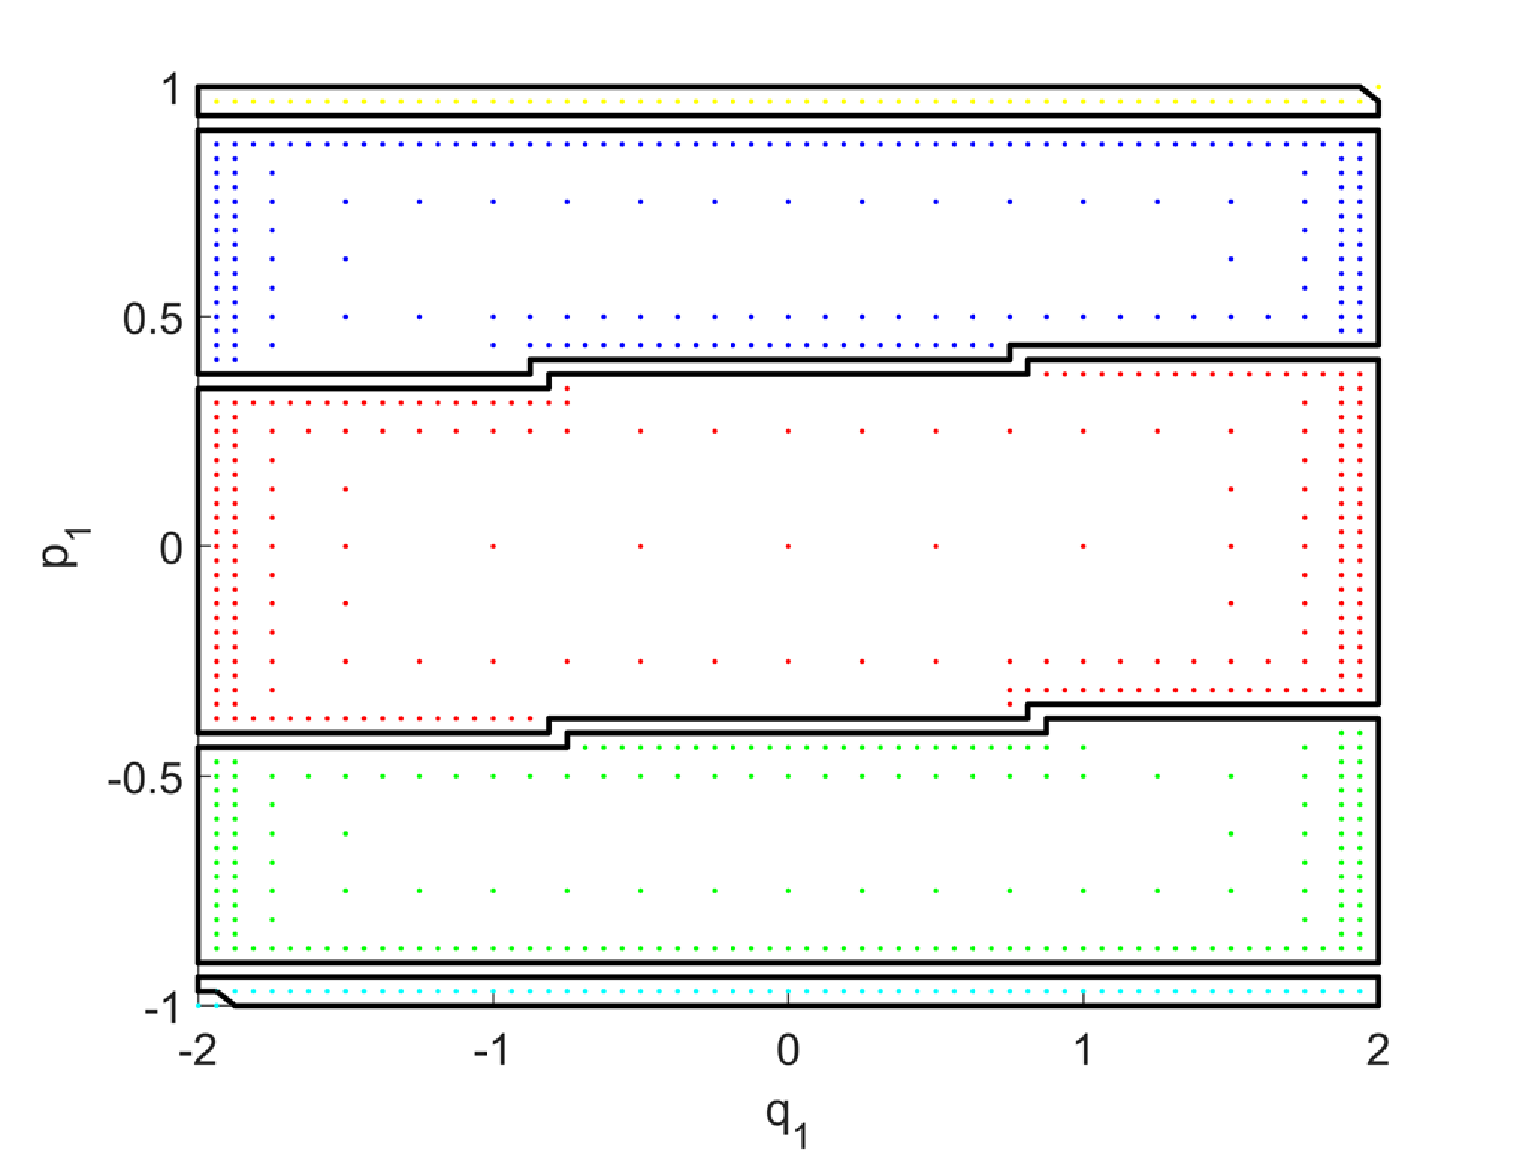
\includegraphics[width=\textwidth]{boundaries_source_triangles2}
 \caption{The black lines are the boundaries at \set{S}{}{}. $1500$ rays are traced using the triangulation refinement with $\varepsilon_{\variabile{q}_1}^{\textrm{min}}=0.1$. }
  \label{fig:boundaries_s2}
\end{subfigure}%
\hfill
\begin{subfigure}{.45\textwidth}
  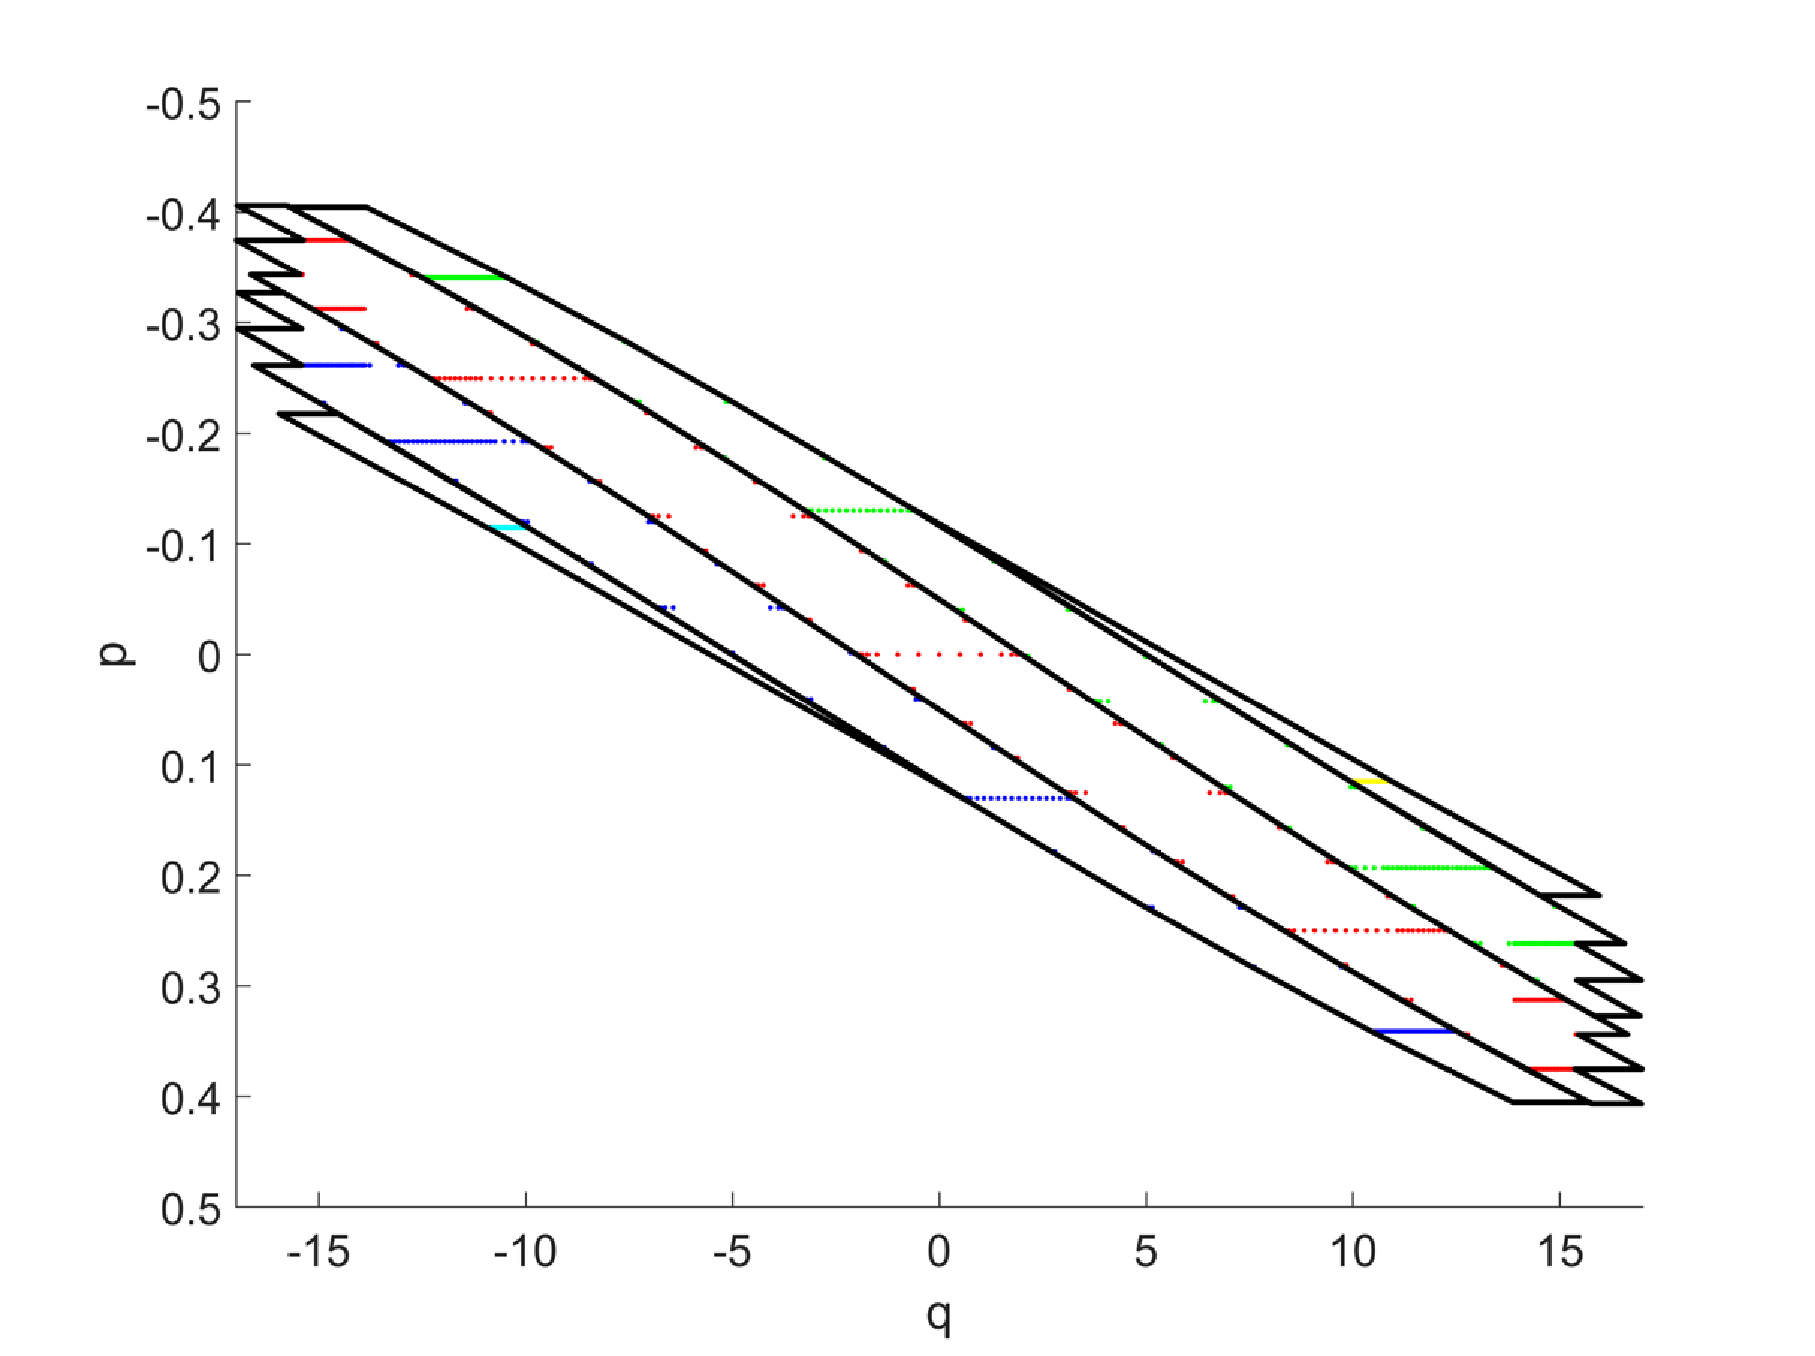
\includegraphics[width=\textwidth]{boundaries_target_triangles2}
  \caption{The black lines are the boundaries at \set{T}{}{}. $1500$ rays are traced using the triangulation refinement with $\varepsilon_{\variabile{q}_1}^{\textrm{min}}=0.1$.} %
  \label{fig:boundaries_t2}
\end{subfigure} %
\hfill
\begin{subfigure}{.45\textwidth}
  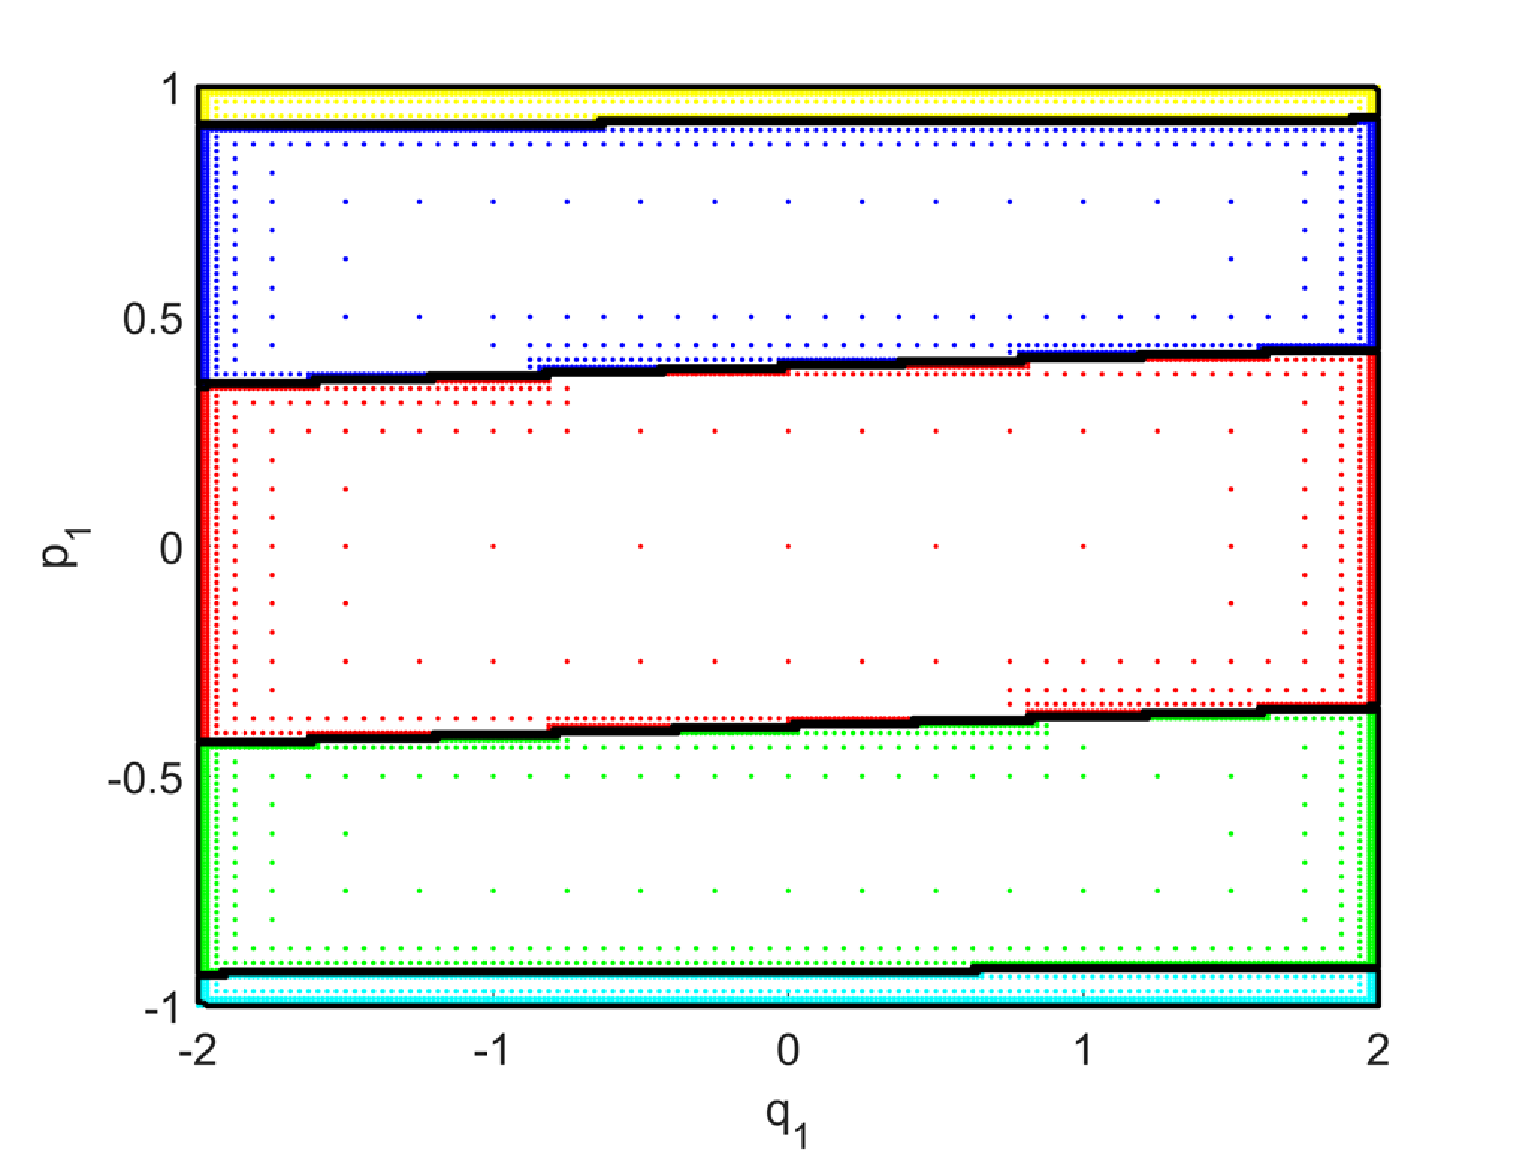
\includegraphics[width = \textwidth]{boundaries_source_triangles1}
  \caption{The black lines are the boundaries at \set{S}{}{}. $7500$ rays are traced using the triangulation refinement with $\varepsilon_{\variabile{q}_1}^{\textrm{min}}=0.025$.}
  \label{fig:boundaries_s1}
\end{subfigure}%
\hfill
\begin{subfigure}{.45\textwidth}
  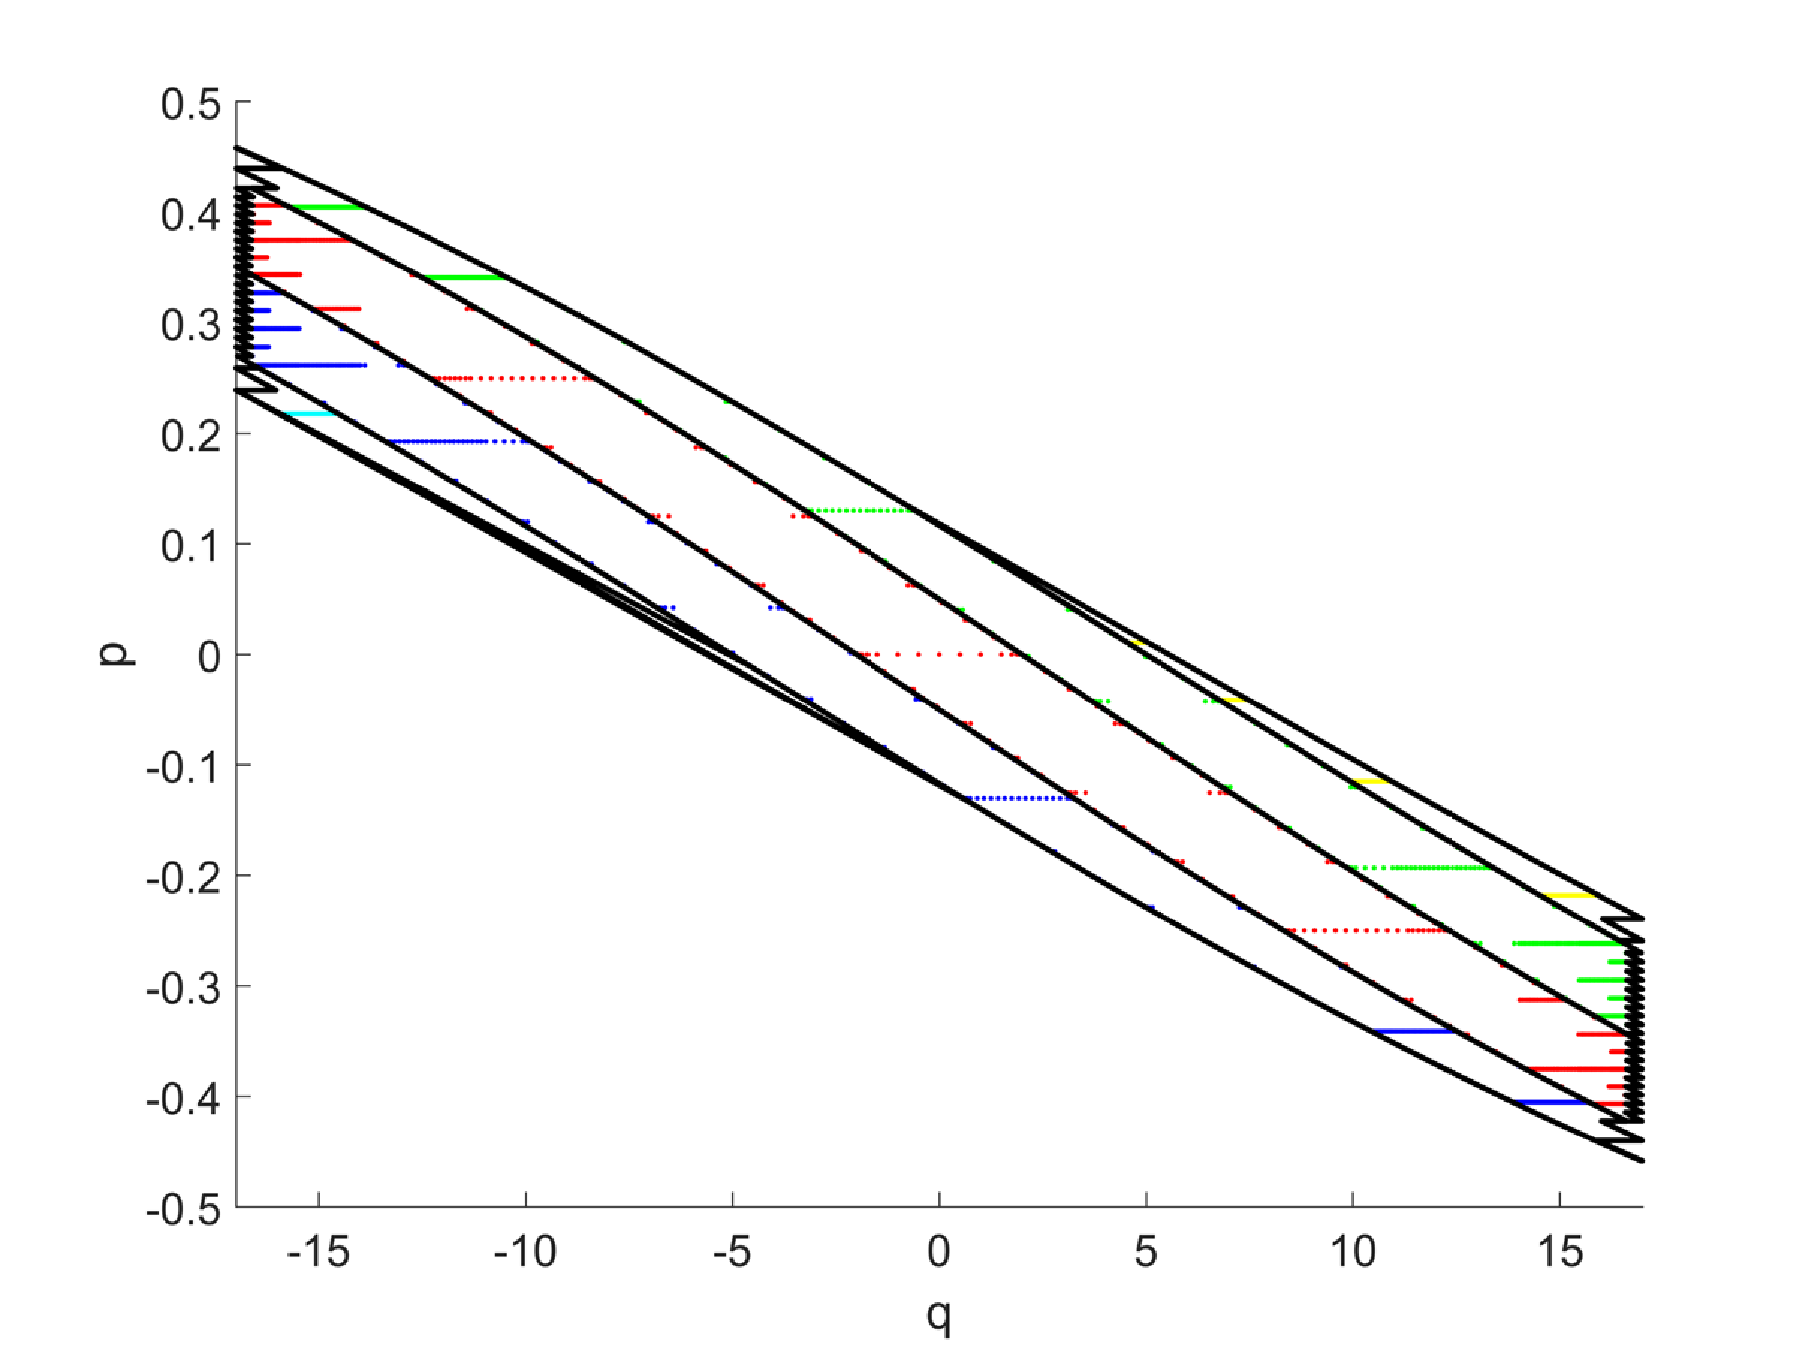
\includegraphics[width=\textwidth]{boundaries_target_triangles1}
 \caption{The black lines are the boundaries at \set{T}{}{}. $7500$ rays are traced using the triangulation refinement with $\varepsilon_{\variabile{q}_1}^{\textrm{min}}=0.025$.} %
  \label{fig:boundaries_t1}
\end{subfigure}
\caption{\textbf{Boundaries at \set{S}{}{} and \set{T}{}{} of the two-faceted cup.} The approximated boundaries are computed using the triangulation refinement with two different values of $\varepsilon_{\variabile{q}_1}^{\textrm{max}}$.}
\label{fig:boundaries_cup}
\end{figure} 
\\ \indent For example, if we consider $\varepsilon_{\variabile{q}_1}^{\textrm{min}}=0.1$, $\varepsilon_{\variabile{q}_1}^{\textrm{max}}=1$ and the corresponding parameters for the $\variabile{p}$-axis given by (\ref{eq:scaled_parameters}), a triangulation with around $1500$ rays (vertices of the triangles) is found. The boundaries $\partial$\set{R}{$1$}{}$(\Pi)$ and $\partial$\set{R}{}{}$(\Pi)$ are calculated using this triangulation refinement and are depicted in black in Figures \ref{fig:boundaries_s2} and \ref{fig:boundaries_t2}, respectively. For this set of rays we found $\Delta U \approx 0.53 $. Next, we can decrease $\varepsilon_{\variabile{q}_1}^{\textrm{min}}$ to obtain a more precise approximation of $U_{\textrm{t}}$. Choosing $\varepsilon_{\variabile{q}_1}^{\textrm{min}} = 0.025$ and $\varepsilon_{\variabile{q}_1}^{\textrm{max}}=1$, a triangulation formed by around $7500$ rays is obtained. The approximated boundaries $\partial$\set{R}{$1$}{}$(\Pi)$ and $\partial$\set{R}{}{}$(\Pi)$ are depicted with black lines in Figures \ref{fig:boundaries_s1} and \ref{fig:boundaries_t1}, respectively. The approximation of the target \'{e}tendue gives $\Delta U \approx 0.13 $.
 Obviously, the boundaries computation obtained using $\varepsilon_{\variabile{q}_1}^{\textrm{min}} = 0.025$ is more accurate. 
Note that, decreasing $\varepsilon_{\variabile{q}_1}^{\textrm{min}}$, the number of rays increases. 
\\ \indent In Figure \ref{fig:etendue_cup} we show with the blue line how the target \'{e}tendue varies as a function of the parameter $\varepsilon_{\variabile{q}_1}^{\textrm{min}}$. The exact \'{e}tendue $U=8$ is depicted with the red line and it is computed using Equation (\ref{eq:etenduetarg1}). By decreasing $\varepsilon_{\variabile{q}_1}^{\textrm{min}}$ an increase of $U_{\textrm{t}}$ is observed. %Furthermore, by construction, $U_{\textrm{t}}$ is always underestimated because the approximated boundaries are found joining the vertices of the \textit{boundaries triangles} which are \textit{inside} the regions \set{R}{}{}$(\Pi)$.
 \begin{figure}[t]
  \center
  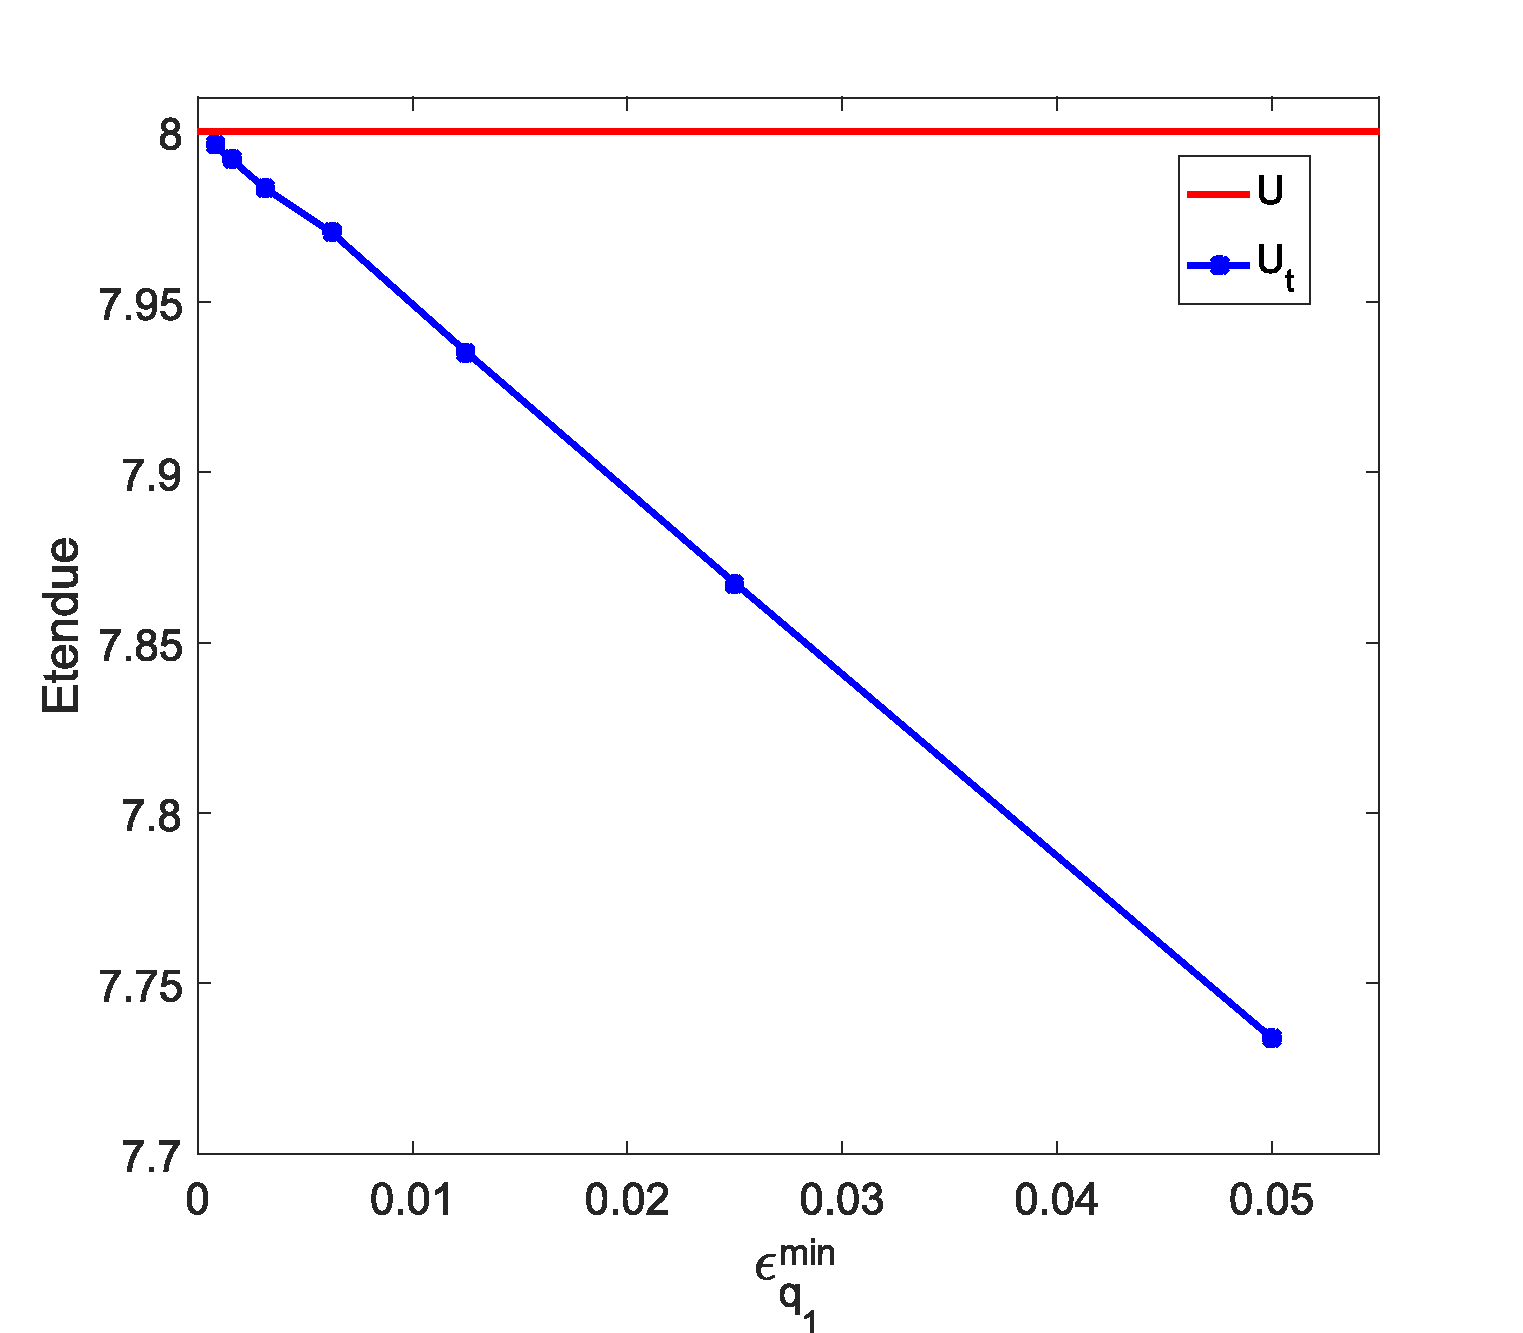
\includegraphics[width= 0.8\textwidth]{etendue_cup_epsilon}
  \caption{\textbf{Etendue for the two-faceted cup.} The total \'{e}tendue as an area in PS is depicted with the red line. The approximated \'{e}tendue for a range of values of 
$\varepsilon_{\variabile{q}_1}^{\textrm{min}}$ is shown with the blue line.}
  \label{fig:etendue_cup}
\end{figure}
In Figure \ref{fig:etendue_cup} we show the approximation of $U_{\textrm{t}}$ for at most around $1.2 \cdot 10^5$ rays traced using PS ray tracing with parameters $\varepsilon_{\variabile{q}_1}^{\textrm{min}}=0.8\cdot 10^{-4}$, $\varepsilon_{\variabile{q}_1}^{\textrm{max}}=1$, $\varepsilon_{\variabile{p}_1}^{\textrm{min}}=\varepsilon_{\variabile{q}_1}^{\textrm{min}}/2$ and $\varepsilon_{\variabile{p}_1}^{\textrm{max}}= \varepsilon_{\variabile{q}_1}^{\textrm{max}}/2$. We expect that further decreasing $\varepsilon_{\variabile{q}_1}^{\textrm{min}}$ the value of $U_{\textrm{t}}$ becomes more precise. 
\\ \indent The PS intensity $\hat{I}_{\textrm{PS}}$ with $1.2 \cdot 10^5$ rays is calculated from Equation (\ref{eta2}). The intensity profile is shown in Figure \ref{fig:intensity_cup_triangulation} with the red line. In the same graph we show the reference intensity $\hat{I}_{\textrm{ref}}$ with the dotted blue line. For the two-faceted cup the reference intensity is actually the exact intensity ($\hat{I}_{\textrm{ref}}= \hat{I}_{\textrm{exact}}$). 
 \begin{figure}[t]
  \center
  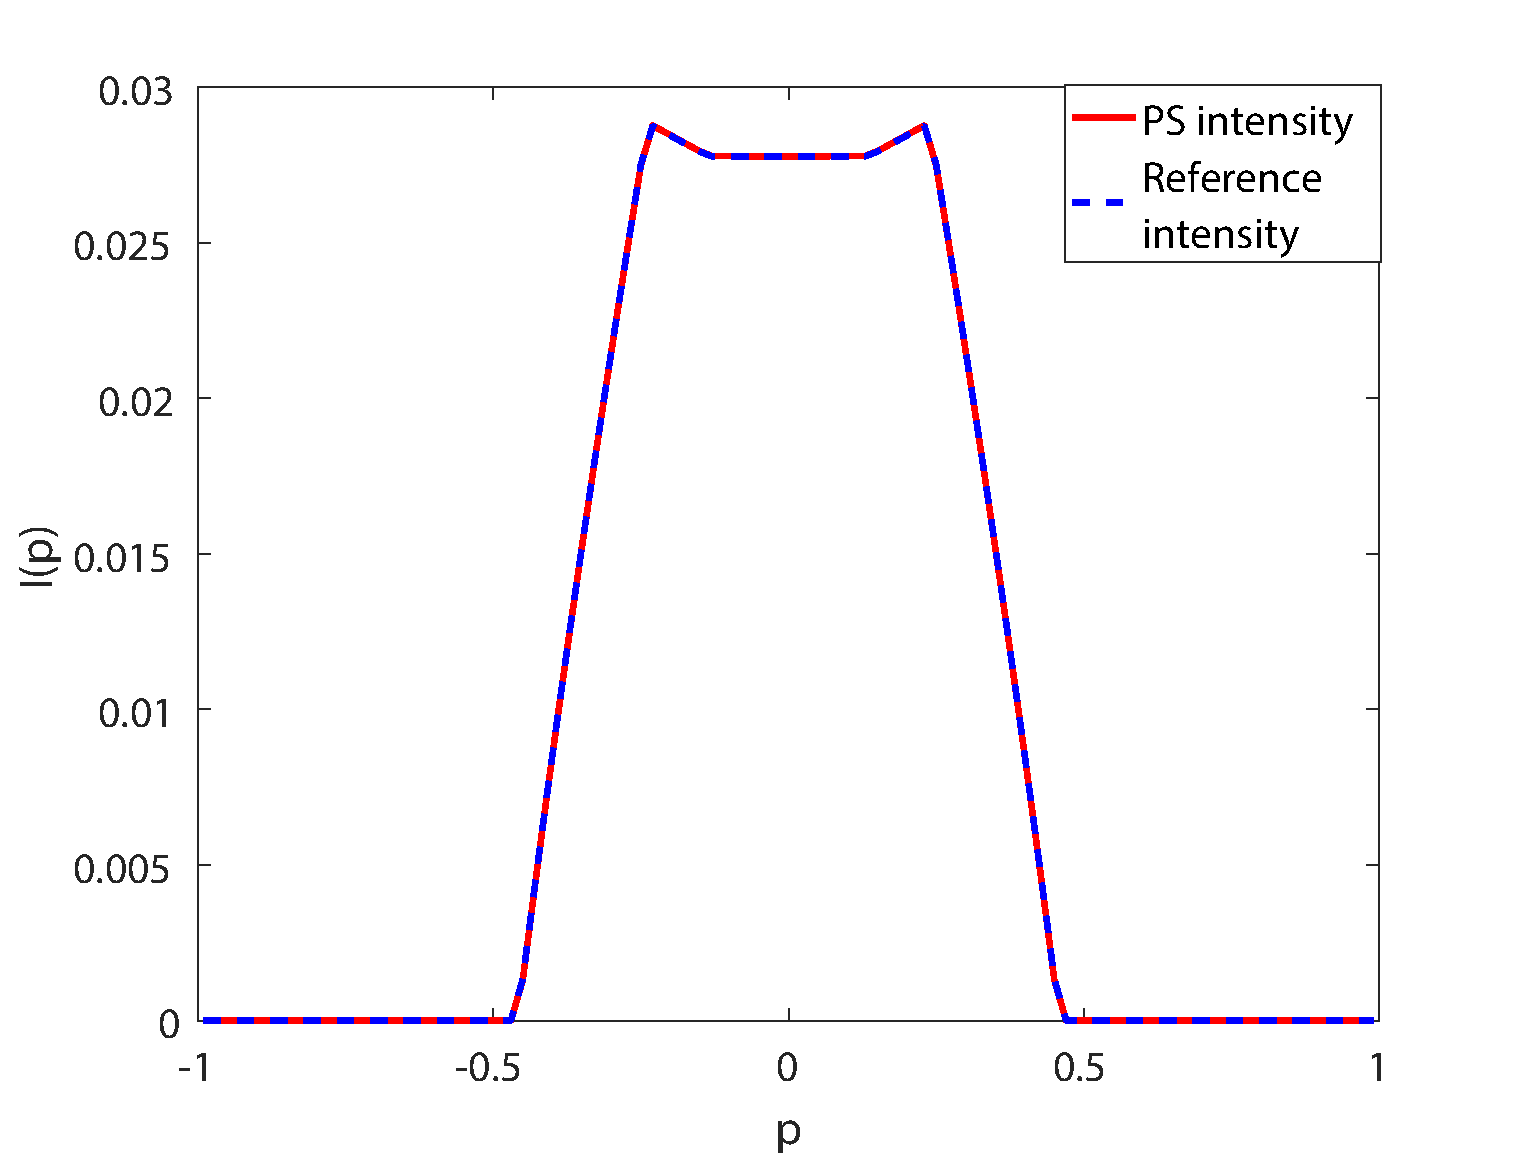
\includegraphics[width= 0.8\textwidth]{intensity_cup_triangulation}
  \caption{\textbf{Intensity profile at the target of the two-faceted cup.} The reference intensity is the exact intensity. The PS intensity is computed using the triangulation refinement with $\varepsilon_{\variabile{q}_1}^{\textrm{min}}=0.8\cdot 10^{-4}$, $\varepsilon_{\variabile{q}_1}^{\textrm{max}}=1$, $\varepsilon_{\variabile{p}_1}^{\textrm{min}}=\varepsilon_{\variabile{q}_1}^{\textrm{min}}/2$ and $\varepsilon_{\variabile{p}_1}^{\textrm{max}}= \varepsilon_{\variabile{q}_1}^{\textrm{max}}/2$. Around $1.2 \cdot 10^5$ rays are traced.}
  \label{fig:intensity_cup_triangulation}
\end{figure}
\\ \indent 
Finally, we compare PS ray tracing with both MC and QMC ray tracing by computing the error between the approximated intensities $\hat{I}_{\textrm{A}}  (\textrm{A}= \textrm{MC}, \textrm{QMC}, \textrm{PS})$ and the exact intensity $\hat{I}_{\textrm{ref}}$ using (\ref{eq:error}). For the error calculation we use (\ref{eq:error}) with $\nbin = 100$. The results are shown in Figure \ref{fig:error_cup_triangulation} where the MC, QMC and PS intensity are depicted with the green, blue and red line, respectively.
 \begin{figure}[t]
  \center
  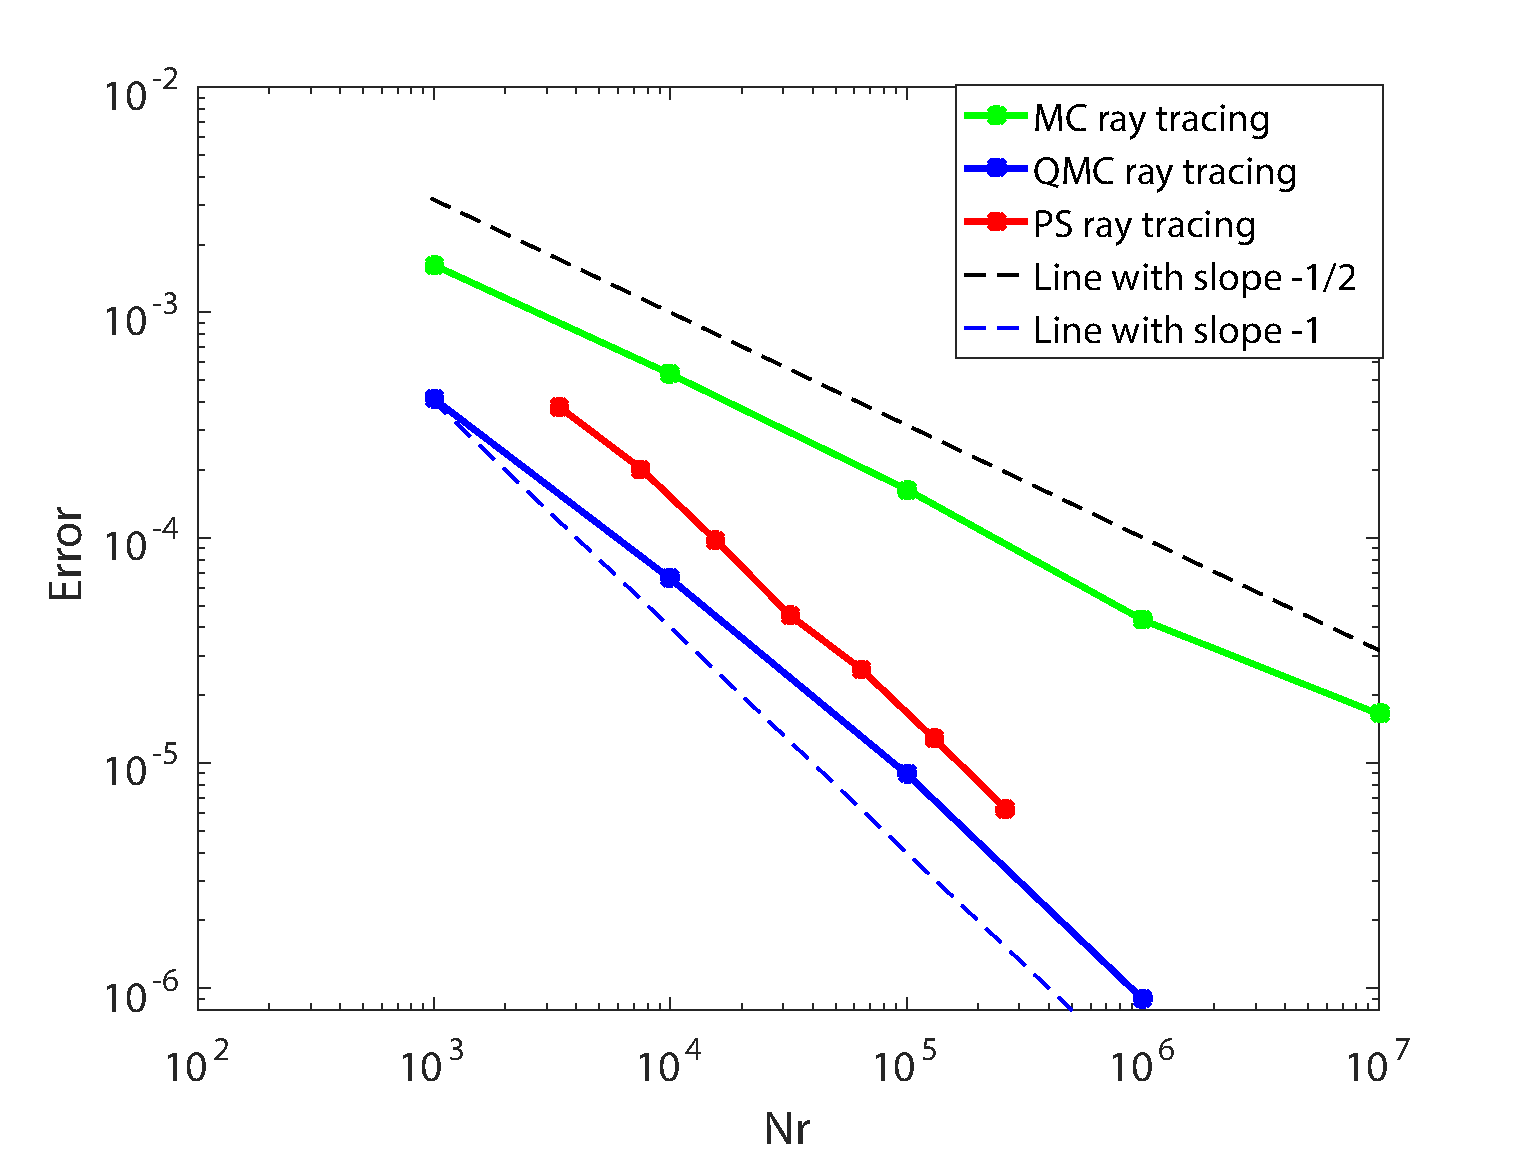
\includegraphics[width= \textwidth]{error_cup_triangulation}
  \caption{\textbf{Error plot for the two-faceted cup.} The errors between the approximated intensities $\hat{I}_{\textrm{A}} (\textrm{A}= \textrm{MC}, \textrm{QMC}, \textrm{PS})$ and the exact intensity $\hat{I}_{\textrm{exact}}$.}
  \label{fig:error_cup_triangulation}
\end{figure}
The graph shows that using PS ray tracing in combination with the triangulation refinement admits tracing far less rays compared to MC ray tracing.
A comparison between QMC ray tracing and PS ray tracing shows that more rays are needed in PS. Indeed, although the shapes of all the regions \set{R}{}{}$(\Pi)$ are very smooth, their boundaries at the edge of the target phase space \set{T}{}{} are difficult to approximate by triangles. With the triangulation refinement, the vertical straight lines at the edge of \set{T}{}{} are always approximated by a broken line. However, the two-faceted cup is a very simple system and QMC ray tracing does not requires a large number of rays to obtain the desired accuracy. \\ \indent Nevertheless, PS ray tracing has a big advantage compared to QMC ray tracing. Indeed, as we have seen in Chapter \ref{chap:raytracing}, MC and QMC ray tracing are binning procedures. Therefore, the MC and QMC intensities are given by the average over every bin and the error also depends on the number of bins. % according to Equations \ref{} \ref{}
PS ray tracing gives a pointwise intensity along all possible directions. In the simulations shown in this thesis we always compute the average PS intensity. This is needed to give a fair comparison of PS ray tracing versus MC and QMC ray tracing. It is very important to observe that no error related to the number of bins is involved in the PS procedure. \\ \indent
To investigate in more detail the performance of PS ray tracing, we test the method for more complicated systems. In the next paragraph we present the results for a TIR-collimator. 
\section{A TIR-collimator}
In this section we provide the results of PS ray tracing for a TIR-collimator, using the triangulation refinement to compute the boundaries $\partial$\set{R}{}{}$(\Pi)$ in target PS. In particular, we consider the TIR-collimator depicted in Figure \ref{fig:analyticlens}. Since this system is located in two different media (air and glass), also the refraction law plays a role in the ray tracing procedure. We run PS ray tracing for the TIR-collimator several times gradually increasing the number of rays, i.e., gradually decreasing the values of the parameters $\varepsilon_{\variabile{q}_1}^{\textrm{min}}, \varepsilon_{\variabile{q}_1}^{\textrm{max}}, \varepsilon_{\variabile{p}_1}^{\textrm{min}}$ and $\varepsilon_{\variabile{p}_1}^{\textrm{max}}$ in the triangulation. In order to trace more rays close to the boundaries, we decide to vary only the values of $\varepsilon_{\variabile{q}_1}^{\textrm{min}}$ and $ \varepsilon_{\variabile{p}_1}^{\textrm{min}}$ while fixing the values of $ \varepsilon_{\variabile{q}_1}^{\textrm{max}}$ and $ \varepsilon_{\variabile{p}_1}^{\textrm{max}}$ as the last two are responsible of the number of rays inside the regions \set{R}{}{}$(\Pi)$. Every ray traced has initial position coordinate $\variabile{q}_1\in[-\variabile{a}, \variabile{a}]$ with $\variabile{a}=2$ and the initial direction coordinate $\variabile{p}_1\in[-1,1]$. Therefore, the source PS of the TIR-collimator is the rectangular domain \set{S}{}{}$= [-2, 2] \times [-1, 1]$. The parameters $\varepsilon_{\variabile{p}_1}^{\textrm{min}}$ and $\varepsilon_{\variabile{p}_1}^{\textrm{max}}$ are scaled as in Equation (\ref{eq:scaled_parameters}).
\\ \indent To determine the triangulation refinement that gives a good approximation of the target intensity we compare $U_1$ (source \'{e}tendue) to $U_{\textrm{t}}$ (target \'{e}tendue) and use \'{e}tendue conservation. In this case, not all light emitted by the source of the TIR-collimator arrives at the target. Indeed, using PS ray tracing, $\npath=7$ different paths $(\Pi_\lineai)_{\lineai=1, \cdots, \npath}$ are found but only five of them are paths from the source (line $1$) to the target (line $12$), see also Section \ref{sec:results-Tir-alpha}. Thus, we need to remove from the total area of \set{S}{}{} those parts occupied by the rays that arrive at some others detectors and not at the target. % white areas in figure...
Indicating with $A_T$ the area of each of these parts (see Section \ref{sec:results-Tir-alpha}), the source PS is given by:
\begin{equation}
U_1 = 8-2A_T\approx 7.77.
\end{equation}
The target \'{e}tendue $U_{\textrm{t}}$ is obtained from Equation (\ref{eq:etenduetarg}) for a range of values of $\varepsilon_{\variabile{q}_1}^{\textrm{min}}$ and for $\varepsilon_{\variabile{q}_1}^{\textrm{max}}=1$ fixed. The boundaries $\partial$\set{R}{}{}$(\Pi)$ are found for every value of $\varepsilon_{\variabile{q}_1}^{\textrm{min}}$ and, $U_{\textrm{t}}$ is calculated for each of these boundaries. 
The results shown in Figure \ref{fig:etendue_tir_triangulation} give the \'{e}tendue plot as a function of $\varepsilon_{\variabile{q}_{1}}^{\textrm{min}}$.
 \begin{figure}[t]
  \center
  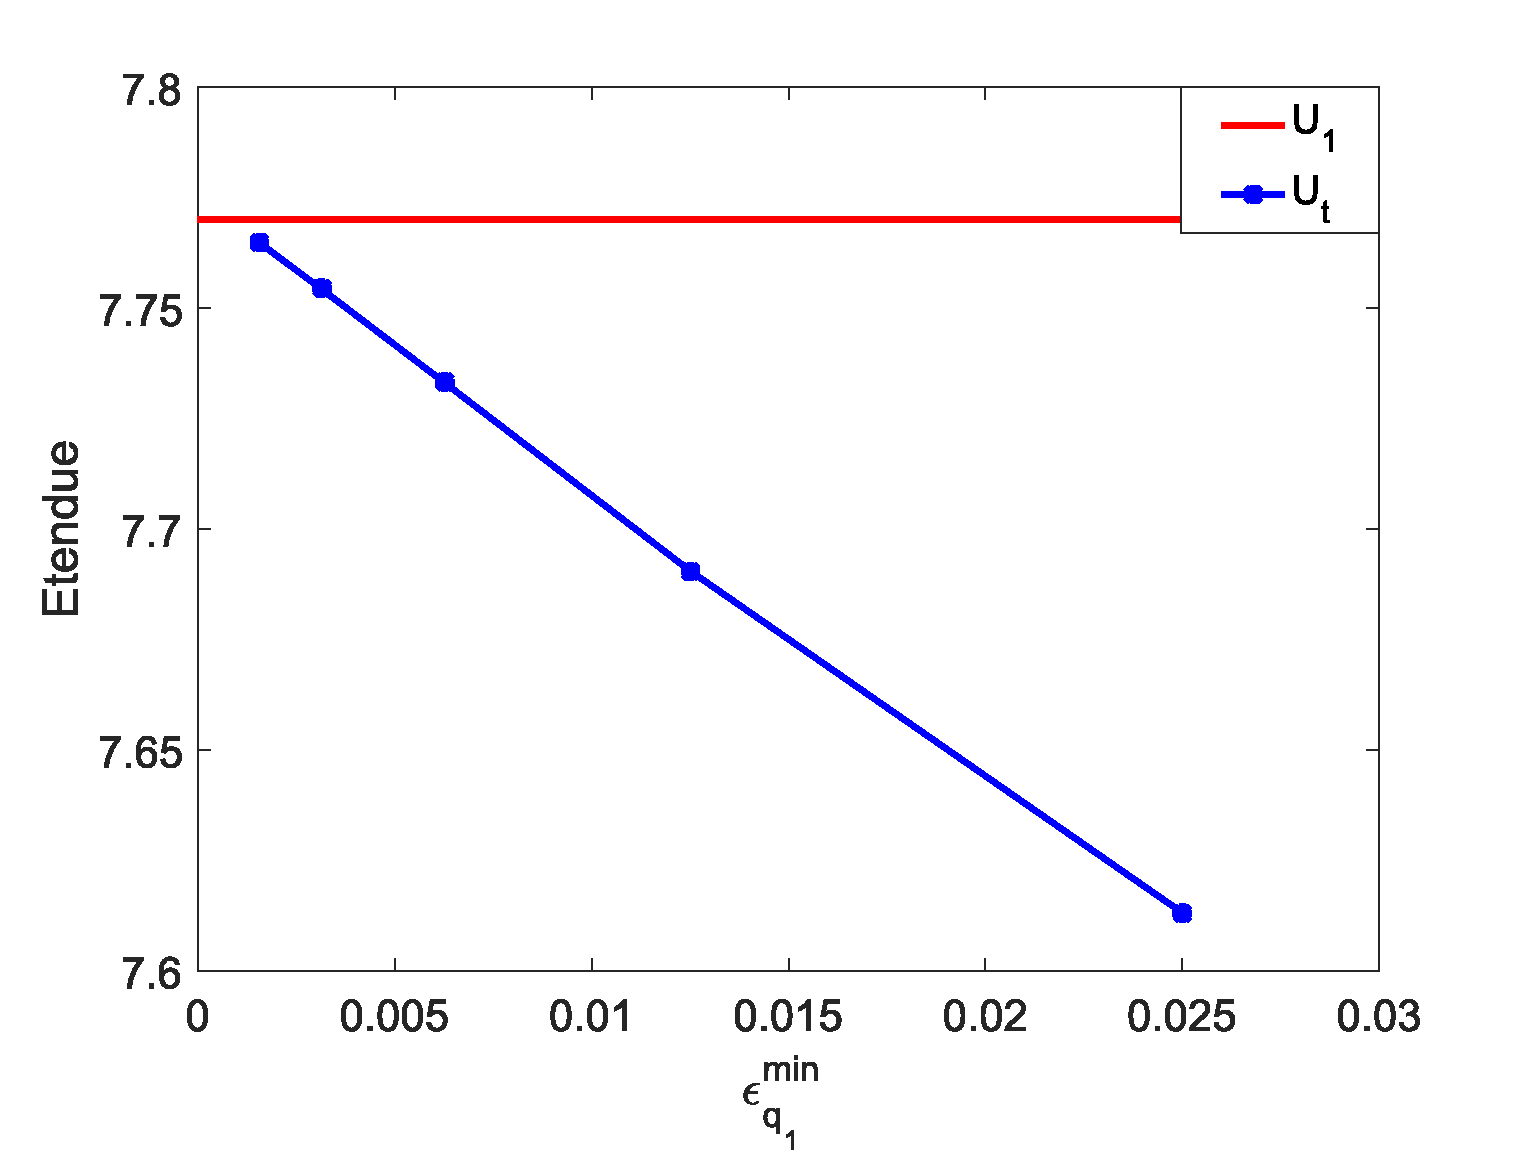
\includegraphics[width = 0.8\textwidth]{etendue_tir_triangulation}
  \caption{\textbf{Etendue of the TIR-collimator.} A comparison between $U_1$ and $U_{\textrm{t}}$ shows that by decreasing the value of $\varepsilon_{\variabile{q}_{1}}^{\textrm{min}}$, $\Delta U= U_1-U_{\textrm{t}}$ decreases.}
  \label{fig:etendue_tir_triangulation}
\end{figure}
\\ \indent 
The best approximation of $U_{\textrm{t}}$ shown in the previous graph is obtained using $\varepsilon_{\variabile{q}_1}^{\textrm{min}}=1.6\cdot 10^{-3}$, tracing around $1.62 \cdot 10^5$ rays. The boundaries $\big(\partial\mbox{\set{R}{$1$}{}}(\Pi_{\lineai})\big)_{\lineai = 1, \cdots, 5}$ and $\big(\partial\mbox{\set{R}{}{}}(\Pi_{\lineai})\big)_{\lineai = 1, \cdots, 5}$ of the regions formed by these rays are shown in Figure \ref{fig:boundaries_TIR_triangulation} with red lines (see also Figure \ref{fig:Tir2} for comparison). 
\begin{figure}[h]
 \begin{subfigure}[t]{0.5\textwidth}
\centering
    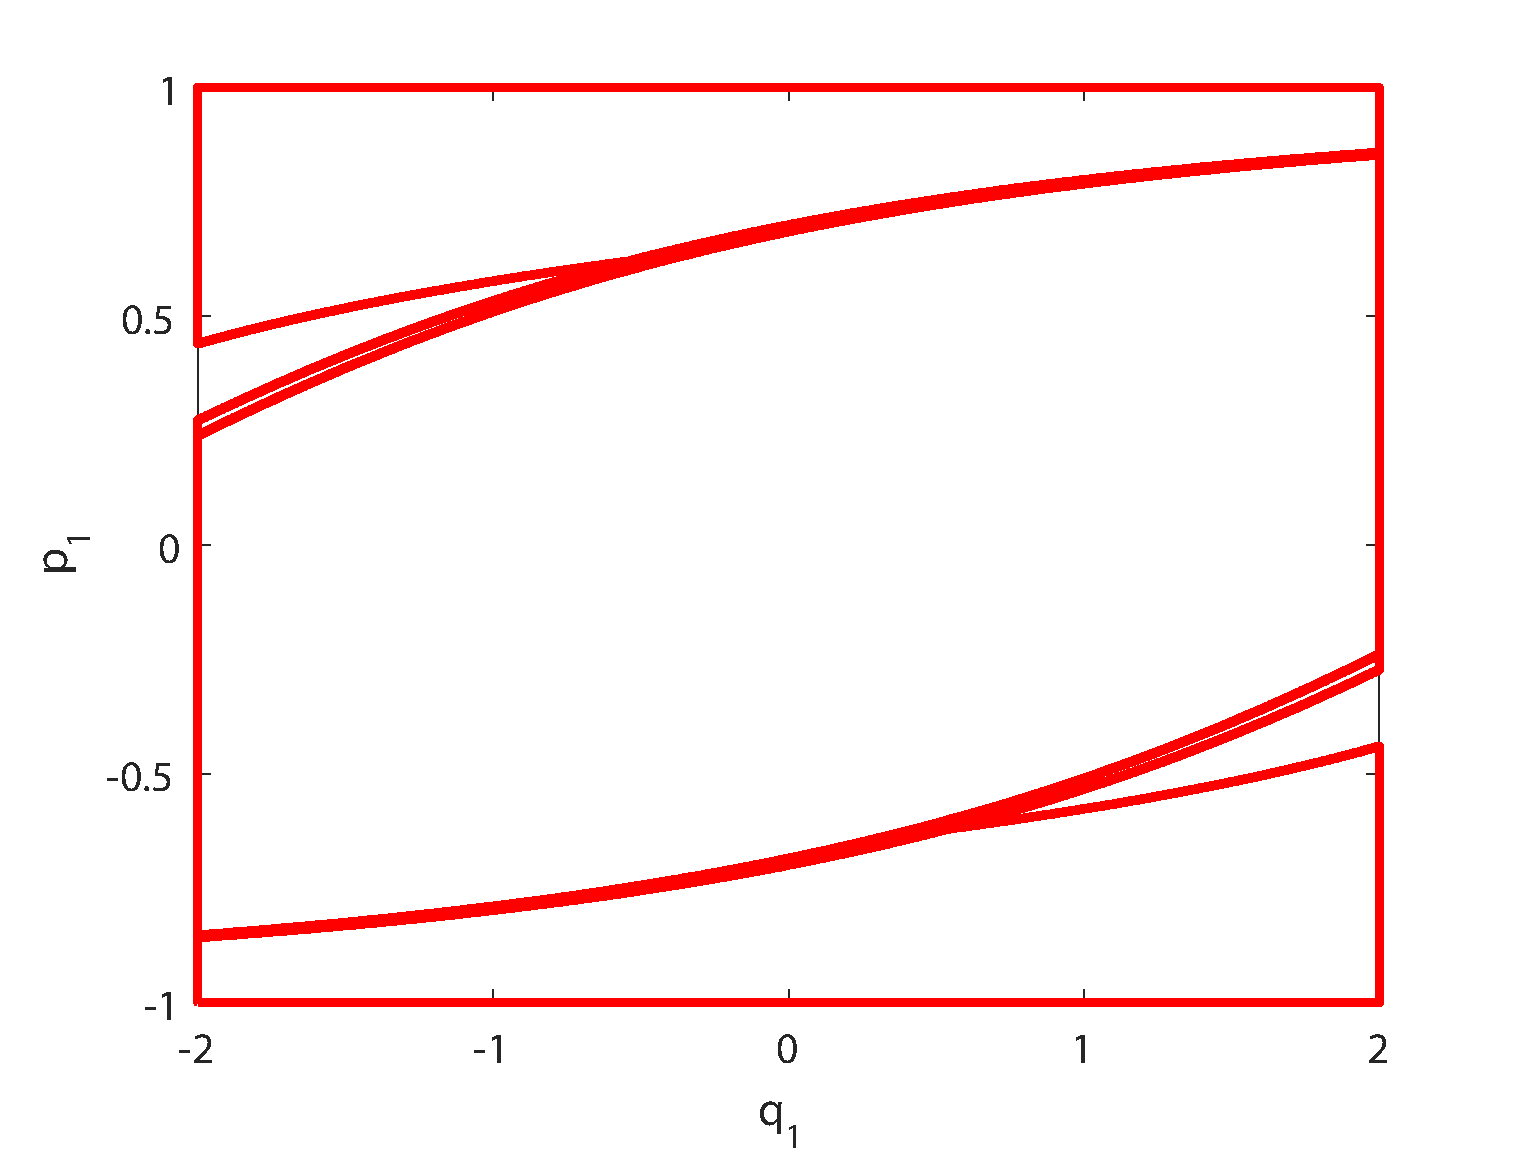
\includegraphics[width=\textwidth]{boundaries_triang_source_tir}
    \caption{Boundaries at the source PS.}
    \label{fig:boundaries_triang_source_tir}
\end{subfigure}
\hfill
\begin{subfigure}[t]{0.5\textwidth}
\centering
    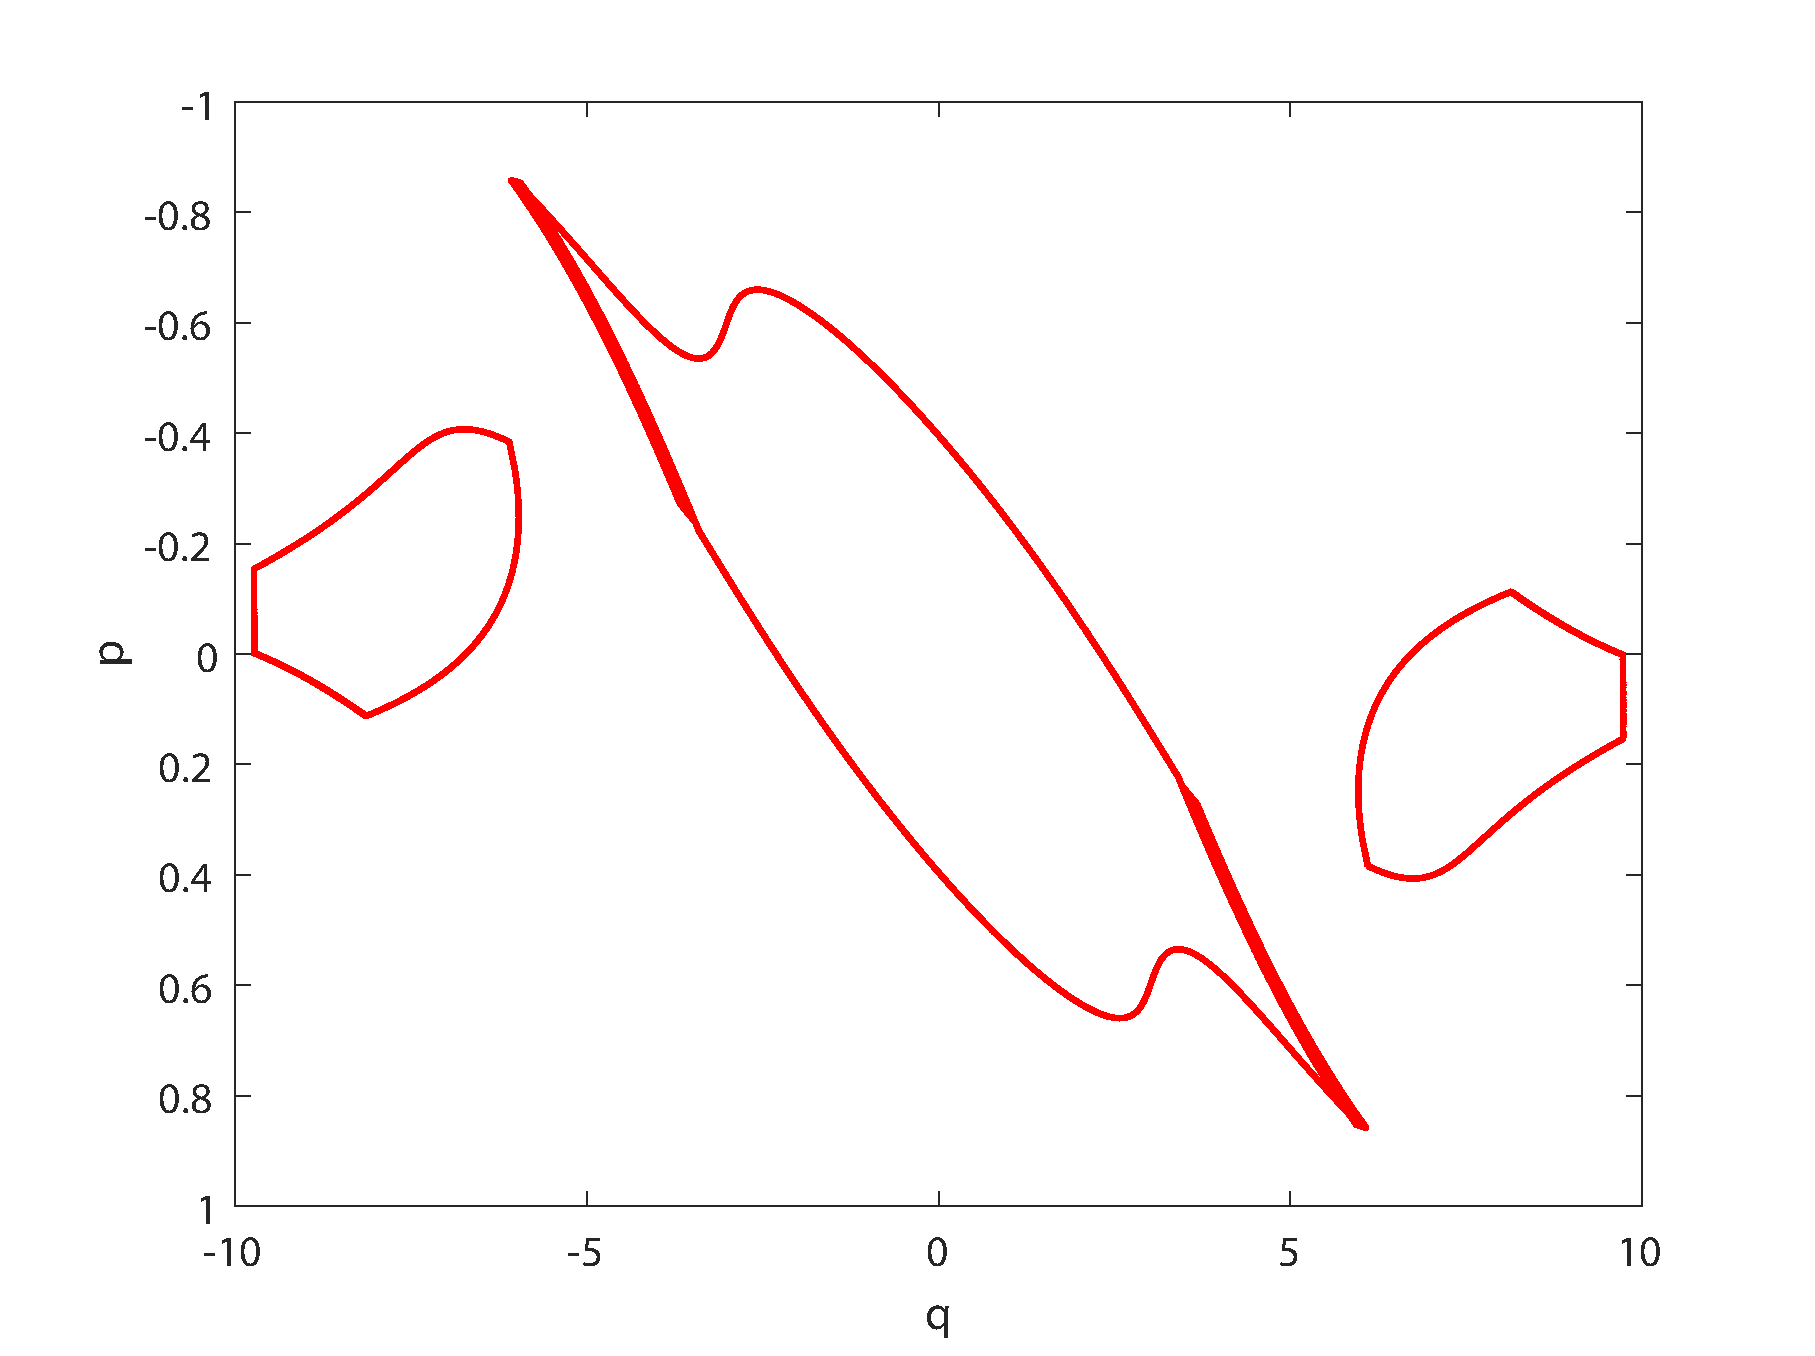
\includegraphics[width = \textwidth]{boundaries_triang_targ_tir}
    \caption{Boundaries at the target PS.}
    \label{fig:boundaries_triang_target_tir}
\end{subfigure}
\caption{\textbf{Boundaries at \set{S}{}{} and \set{T}{}{} of the TIR-collimator.} The red lines show the boundaries found using $\varepsilon_{\variabile{q}_1}^{\textrm{min}}=1.6\cdot 10^{-3}, \varepsilon_{\variabile{q}_1}^{\textrm{max}}=1, \varepsilon_{\variabile{p}_1}^{\textrm{min}}=\varepsilon_{\variabile{q}_1}^{\textrm{min}}/2$ and $\varepsilon_{\variabile{p}_1}^{\textrm{max}} = \varepsilon_{\variabile{q}_1}^{\textrm{max}}/2$.}
 \label{fig:boundaries_TIR_triangulation}
\end{figure}
 \\ \indent 
The target PS intensity $\hat{I}_{\textrm{PS}}$ is computed and is compared with a reference intensity $\hat{I}_{\textrm{ref}}$ which is given by QMC ray tracing with $10^7$ rays (as the exact intensity for the TIR-collimator is unknown). The profile of the two intensities is given in Figure \ref{fig:intensity_tir_triangulation}.
 \begin{figure}[ht]
  \center
  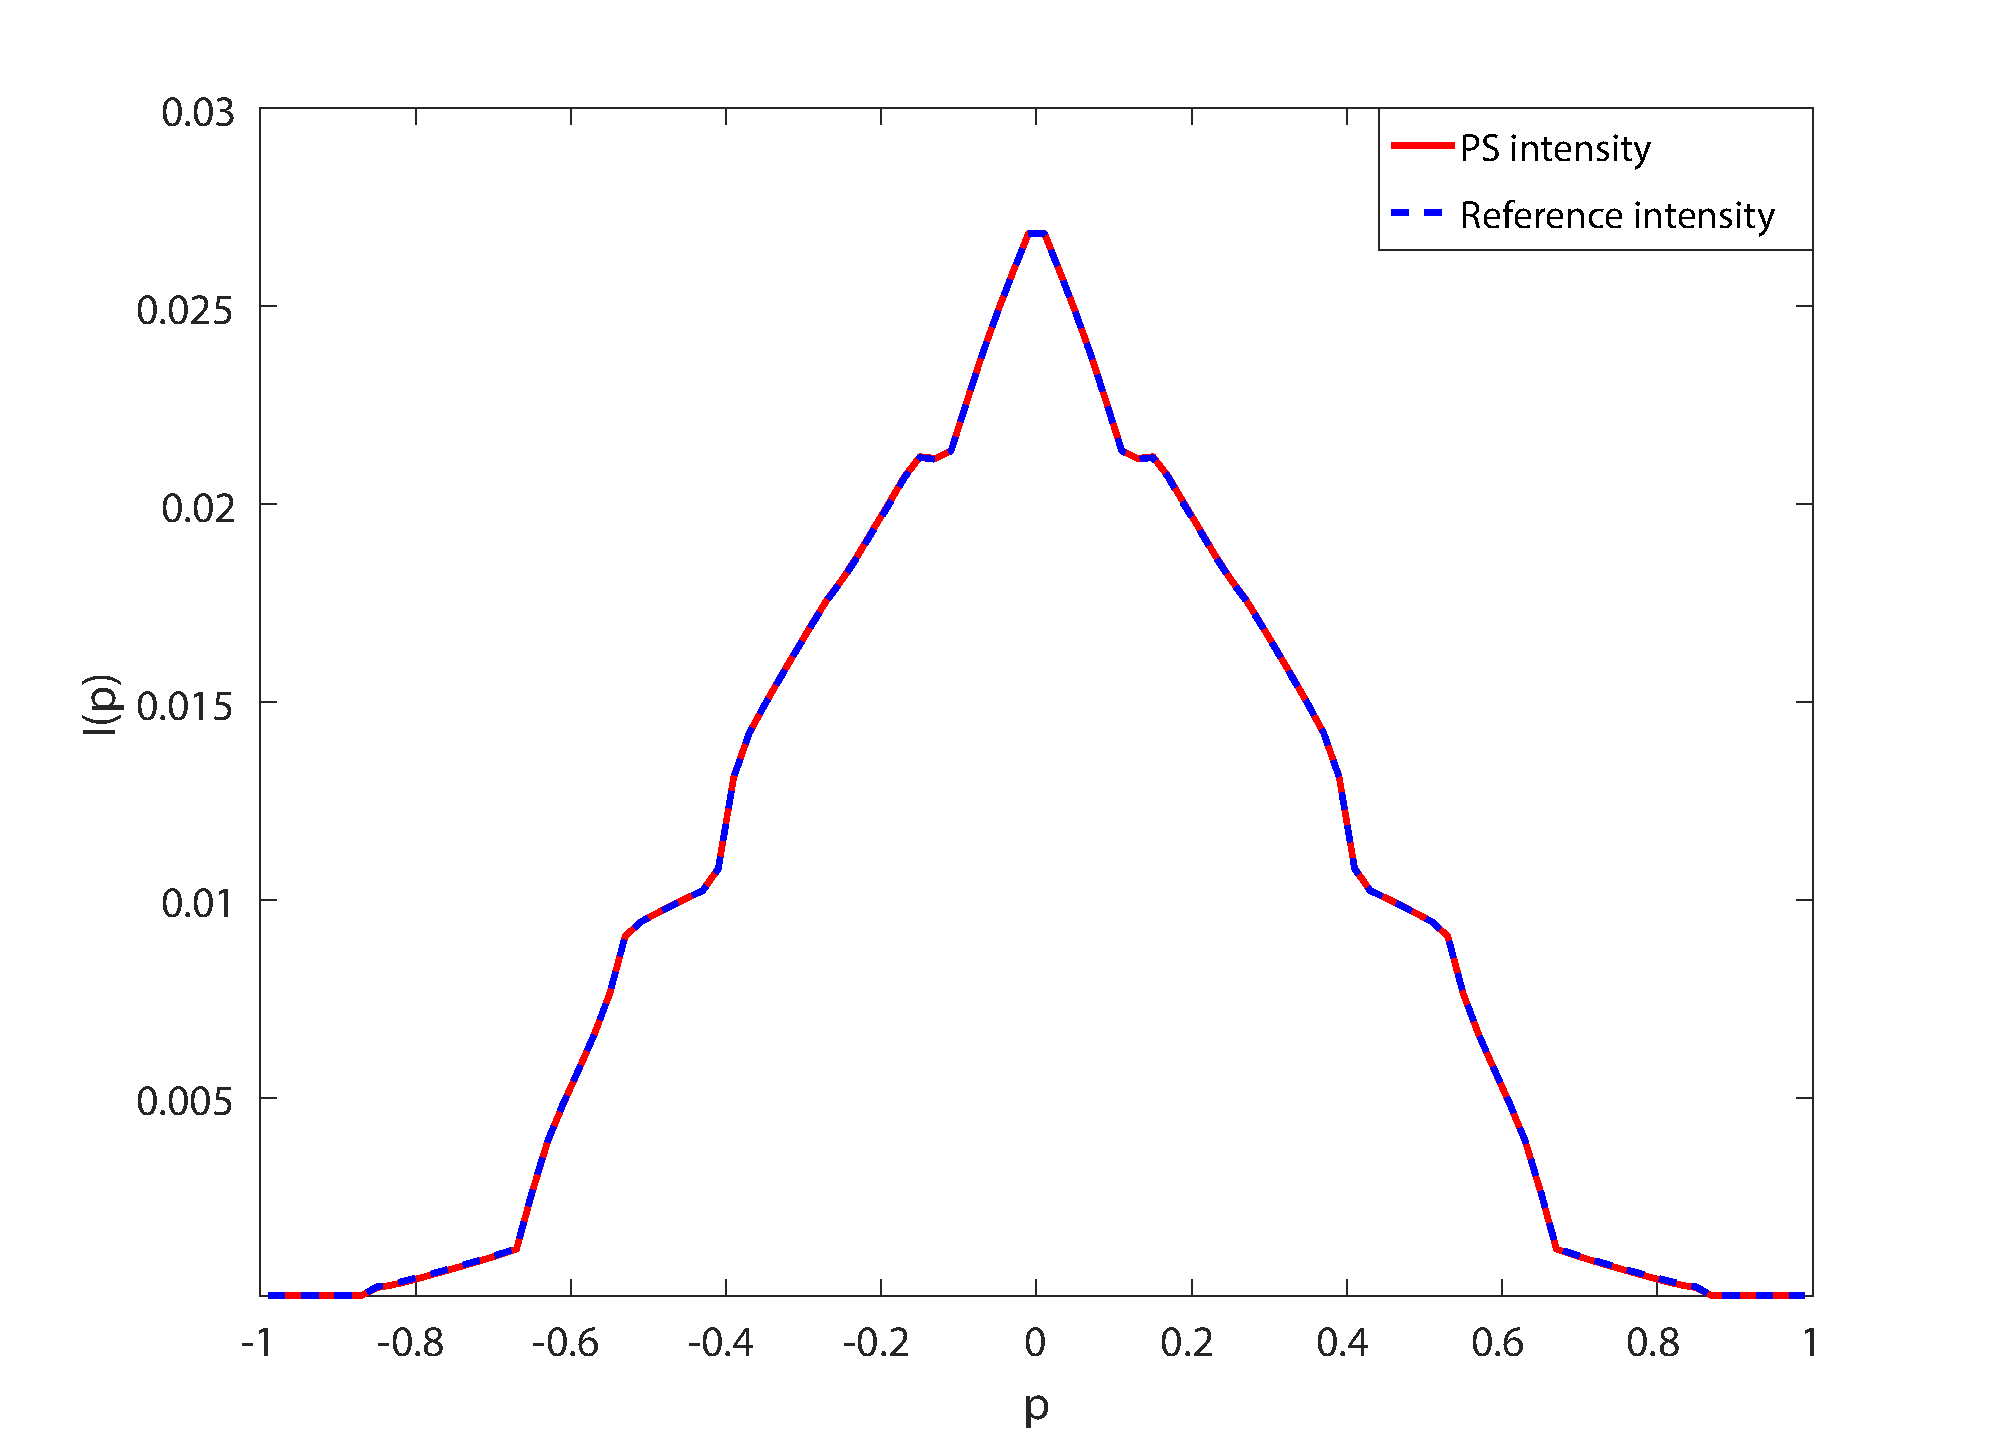
\includegraphics[width= 0.8\textwidth]{intensity_tir_triangulation}
  \caption{\textbf{Target intensity for the TIR-collimator.} The PS intensity $\hat{I}_{\textrm{PS}}$ is computed using PS ray tracing with around $1.62\cdot 10^5$ rays. The reference intensity $\hat{I}_{\textrm{ref}}$ is obtained by QMC ray tracing with $10^7$ rays.}
  \label{fig:intensity_tir_triangulation}
\end{figure}
\\ \indent
To validate our method, PS ray tracing is compared to both MC and QMC ray tracing. The error between the approximated intensities $\hat{I}_{\textrm{A}} (\textrm{A}=\textrm{QMC}, \textrm{MC}, \textrm{PS})$ and the reference intensity $\hat{I}_{\textrm{ref}}$ as a function of the number of rays traced is calculated. The error plot is shown in a logarithmic scale in Figure \ref{fig:error_tir_triangulation} where the MC, QMC and PS convergences are shown with the green, the blue and the red line, respectively. The black dotted line is a line with slope $-\frac{1}{2}$, the blue dotted line has slope $-1$.The graph shows that MC ray tracing converges, for $\nrays \rightarrow \infty$, with an order of $\mathcal{O}\big(\frac{1}{\sqrt{\nrays}}\big)$, while both PS and QMC ray tracing have a speed of convergence of the order $\mathcal{O}\big(\frac{1}{\nrays}\big)$. 
Note that PS ray tracing allows tracing $10^2$ times less rays compared to MC ray tracing and almost $10$ times less rays compared to QMC ray tracing to obtain an error of $10^{-4}$.
 \begin{figure}[h!]
  \center
  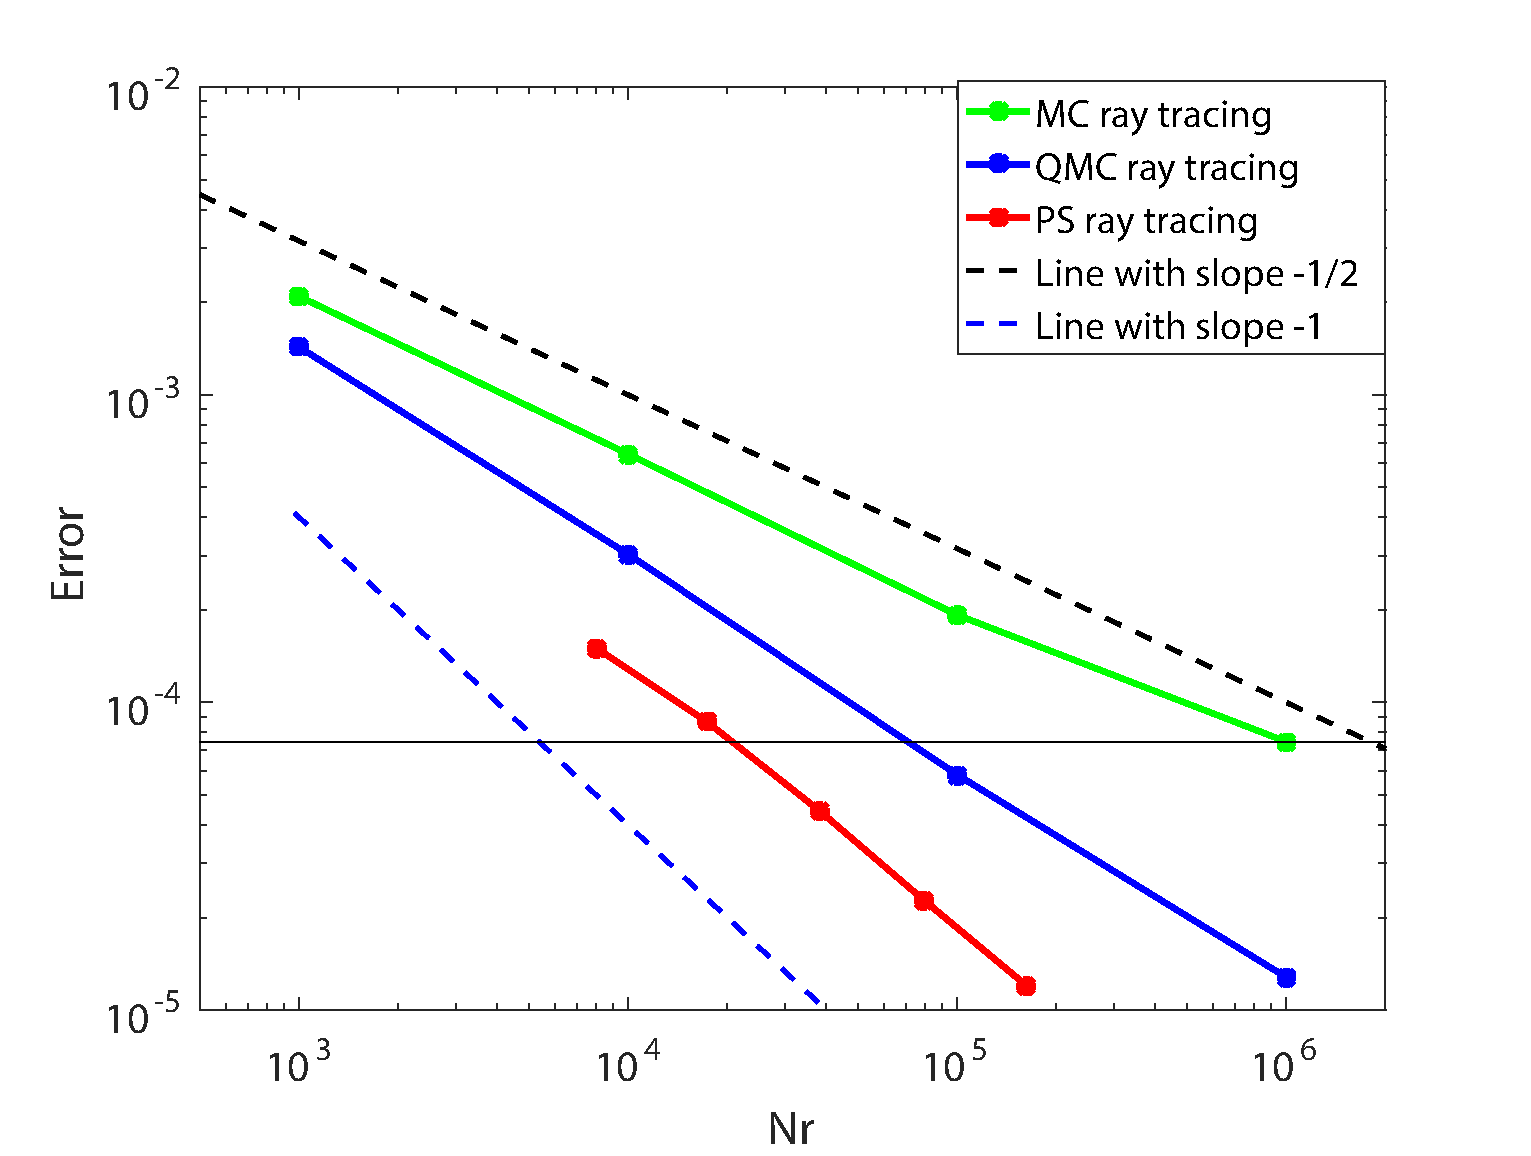
\includegraphics[width= \textwidth]{error_nr_triangulation_tir}
  \caption{\textbf{Error as a function of the number of rays for the TIR-collimator.} The reference intensity $\hat{I}_{\textrm{ref}}$ is obtained by QMC ray tracing with $10^7$ rays.}
  \label{fig:error_tir_triangulation}
\end{figure}
\begin{figure}[h!]
  \center
  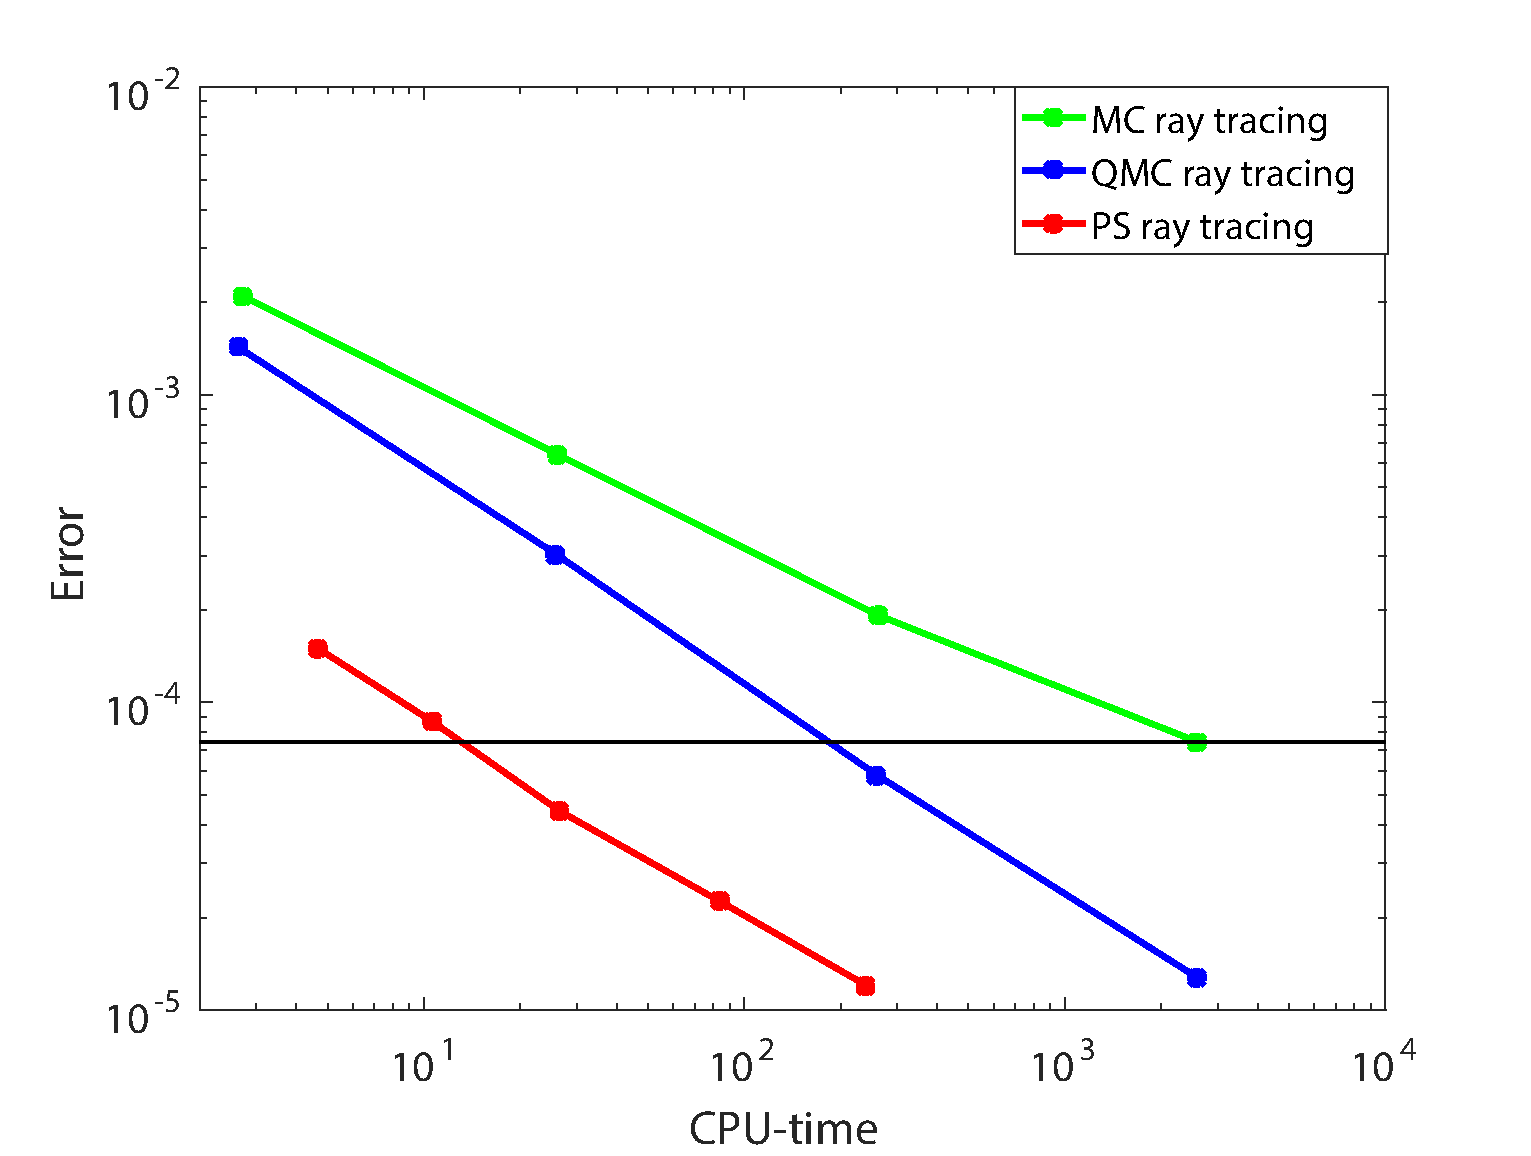
\includegraphics[width= \textwidth]{error_tir_triangulation_time}
  \caption{\textbf{Error as a function of the CPU-time for the TIR-collimator.} The reference intensity $\hat{I}_{\textrm{ref}}$ is obtained by QMC ray tracing with $10^7$ rays.}
  \label{fig:error_tir_triangulation_time}
\end{figure}
\\ \indent Finally, in order to show the advantages of PS ray tracing in terms of the computational time, we provide an error convergence as a function of the CPU-time for all the three methods (MC, QMC and PS raytracing) shown in Figure \ref{fig:error_tir_triangulation_time}. The choice of the colors is consistent with Figure \ref{fig:error_tir_triangulation}. We observe that PS ray tracing outperforms both MC and QMC ray tracing. PS ray tracing is approximately $10^2$ times faster than MC ray tracing and $10$ times faster than QMC ray tracing. \\ \indent The results shown in Figures \ref{fig:error_tir_triangulation} and \ref{fig:error_tir_triangulation_time} are reported in Tables \ref{tab:ps_error_triangulation} and \ref{tab:mc_error_triangulation}.
\begin{table}[t] 
\centering
\caption{\bf Errors of the PS intensity for the TIR-collimator}
\begin{tabular}{lllll}
 \hline   $\varepsilon_{\variabile{q}}^{\textrm{max}} $  & $\nrays$ & Etendue & PS error & PS CPU-time (sec.) \\
  \hline 
 $0.05$ & $3\,547$   & $7.50$   &  $1.75\cdot10^{-4}$ & $1.98$\\
$0.025$  & $8\,055$    & $7.61$    & $1.49\cdot 10^{-4}$ & $4.69$ \\
$0.125$  & $17\,300$    & $7.69$  & $8.68\cdot 10^{-5}$ & $10.61$\\
 $6.3 \cdot 10^{-3}$  & $38\,300$  & $7.73$   & $4.43\cdot 10^{-5}$ & $26.56$\\
 $3.1 \cdot 10^{-3}$ & $79\,600$  & $7.75$    & $2.27\cdot 10^{-5}$ & $83,21$\\
$1.6 \cdot 10^{-3}$ & $162\,300$  & $7.76$    & $1.20\cdot 10^{-5}$ & $240.53$\\
 \hline
 \end{tabular}
\label{tab:ps_error_triangulation}
 \end{table}
\begin{table}[t] \label{tab:table_tir_triangulation}
\centering
\caption{\bf Errors of the MC and QMC intensities for the TIR-collimator}
\begin{tabular}{lllll}
 \hline   $\nrays$ & MC error & MC CPU-time (sec.) & QMC error  & QMC CPU-time (sec.)\\
  \hline 
 $10^3$     & $2.09\cdot 10^{-3}$ & $2.73$ & $1.43\cdot10^{-3}$    & $2.63$\\
 $10^4$     & $6.42\cdot 10^{-4}$ & $25.98$ & $3.03\cdot 10^{-4}$   & $25.84$\\
 $10^5$     & $1.92\cdot 10^{-4}$ & $259.92$ & $5.82\cdot 10^{-5}$   & $258.28$\\
 $10^6$     & $7.45\cdot 10^{-5}$ & $2585.83$   & $1.28\cdot 10^{-5}$   & $2482.67$\\
 \hline
 \end{tabular}
 \label{tab:mc_error_triangulation}
 \end{table}
%\begin{table}[t] 
%\centering
%\caption{\bf Errors of the QMC intensity for the TIR-collimator}
%\begin{tabular}{lllll}
% \hline  $\nrays$\;  & QMC error  & CPU-time (sec.)\\
%  \hline 
% $10^3$   & $1.43\cdot10^{-3}$    & $2.63$  \\
%$10^4$    & $3.03\cdot 10^{-4}$   & $25.84$   \\
%$10^5$    & $5.82\cdot 10^{-5}$   & $258.28$  \\
% $10^6$   & $1.28\cdot 10^{-5}$   & $2482.67$  \\
% \hline
% \end{tabular}
% \label{tab:qmc_error_triangulation}
% \end{table}
%Using PS ray tracing an error equal to $10^{-4}$ is achieved tracing almost $10$ time less compared to QMC ray tracing and $100$ times less rays compared to QMC ray tracing. 
Next, we show the result for a system in which more than $5$ paths are possible. 
In particular we present the results for an optical system for which multiple reflections between rays and the mirrors occur.
\section{A Parabolic reflector}
In this section we show an example of a parabolic reflector which is depicted in Figure \ref{fig:PR}.
 It consists of a source \point{S} (line $1$), a target \point{T} (line $4$) parallel to \point{S} and two reflectors (lines $2$ and $3$) which are arcs of the same parabola. 
  The minimum of the parabola is located at the point with $\variabile{x}$-coordinate equal to $0$. $\point{S}=[\variabile{-a}, \variabile{a}]$ (with $\variabile{a}=2$) and $\point{T}=[-\variabile{b},\variabile{b}]$ (with $\variabile{b}=17$) are lines perpendicular to the optical axis (\variabile{z}-axis) and are located at $\variabile{z}=0$ and $\variabile{z}=40$, respectively.
All the optical lines are located in air, therefore the index of refraction ${n}=1$ for every line.
The optical axis of the system in Figure \ref{fig:PR} corresponds to the \variabile{z}-axis.
\begin{figure}[h!]
\centering
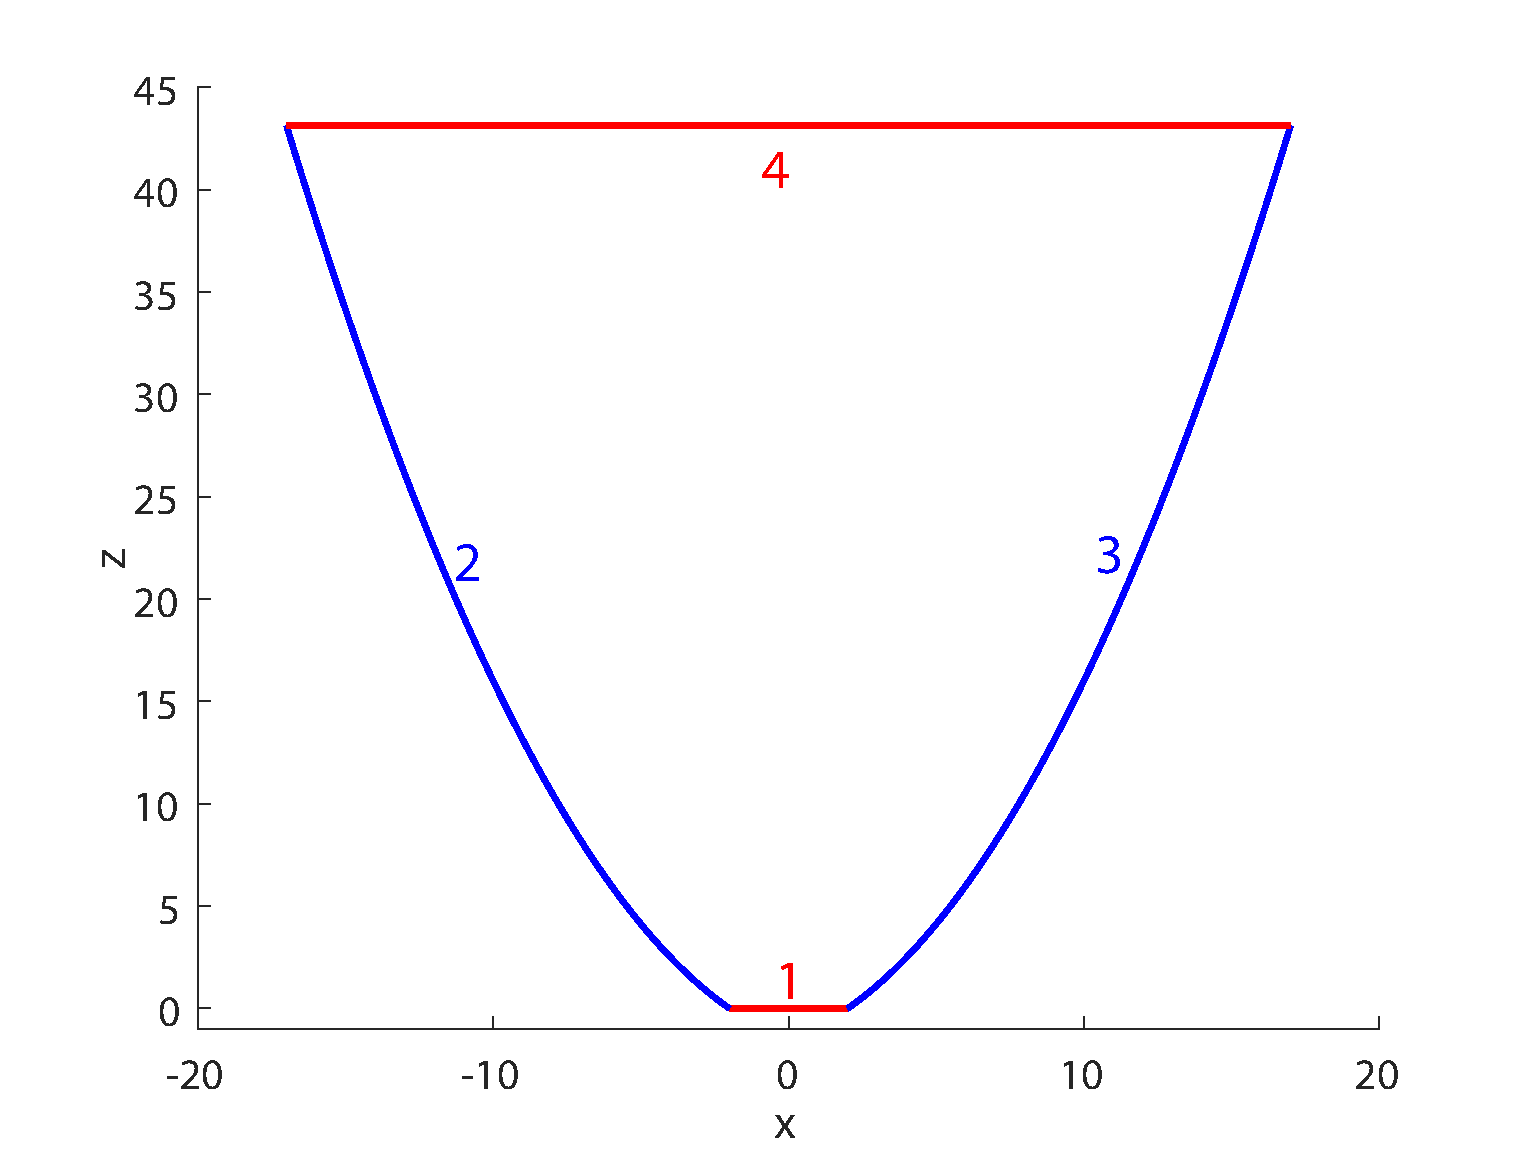
\includegraphics[width=0.7\textwidth]{parabolic_reflector}
\caption{\textbf{A parabolic reflector.}  Each line of the system is labeled with a number.
   The source \point{S}$= [2,2]$ (line $1$) is located on the $\variabile{x}$-axis.
   The target \point{T}$= [-17, 17]$ (line $4$) is parallel to the source and is located at a height $ \variabile{z}= 40$.
   The left and right reflectors (lines $2$ and $3$) are arcs of the same parabola.}
\label{fig:PR}
\end{figure}
We trace rays in PS with source direction coordinates $\variabile{p}_1 \in [-1,1]$ and source position coordinates $\variabile{q}_1\in[-\variabile{a}+\varepsilon,\variabile{a}-\varepsilon]$ where $\varepsilon>0$ is a small number. In particular we take $\varepsilon = 10^{-12}$.\\ \indent As an example we show the triangulation refinement obtained for the parameters $$\varepsilon_{\variabile{q}_1}^{\textrm{min}} = 0.025, \; \varepsilon_{\variabile{q}_1}^{\textrm{max}} = 0.5, \; \varepsilon_{\variabile{p}_1}^{\textrm{min}} = \varepsilon_{\variabile{q}_1}^{\textrm{min}}/2, \mbox{ and }  \varepsilon_{\variabile{p}_1}^{\textrm{max}} = \varepsilon_{\variabile{q}_1}^{\textrm{max}}/2, $$ for which around $8300$ rays are traced in PS. Their distribution at \set{S}{}{} and \set{T}{}{} is shown in Figures \ref{fig:source_triang_pr} and \ref{fig:target_triang_pr}, respectively. 
\begin{figure}[h]
 \begin{subfigure}[h]{0.47\textwidth}
\centering
    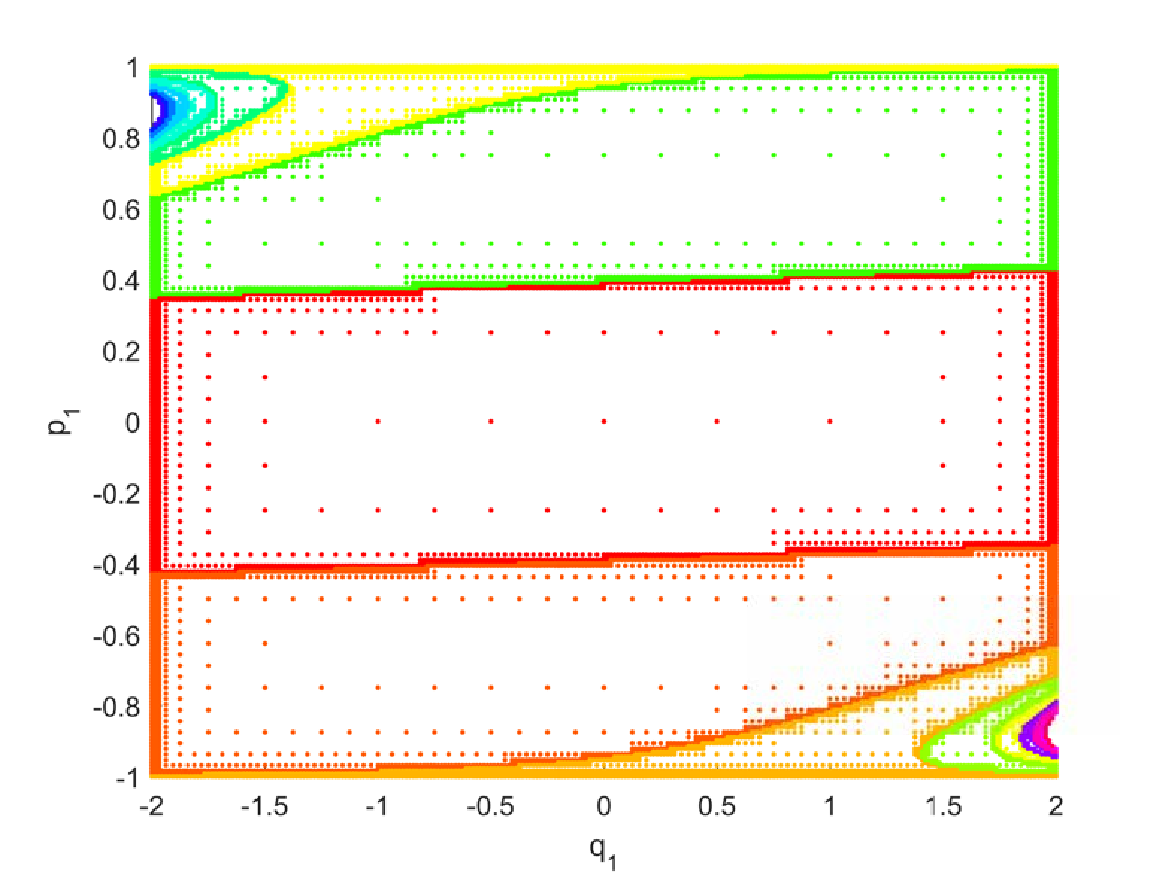
\includegraphics[width=\textwidth]{pr_source}
    \caption{Source PS \set{S}{}{} $= [-\variabile{a}+\varepsilon,\variabile{a}-\varepsilon]\times[-1,1]$}
    \label{fig:source_triang_pr}
\end{subfigure}
\hfill
\begin{subfigure}[h]{0.47\textwidth}
\centering
    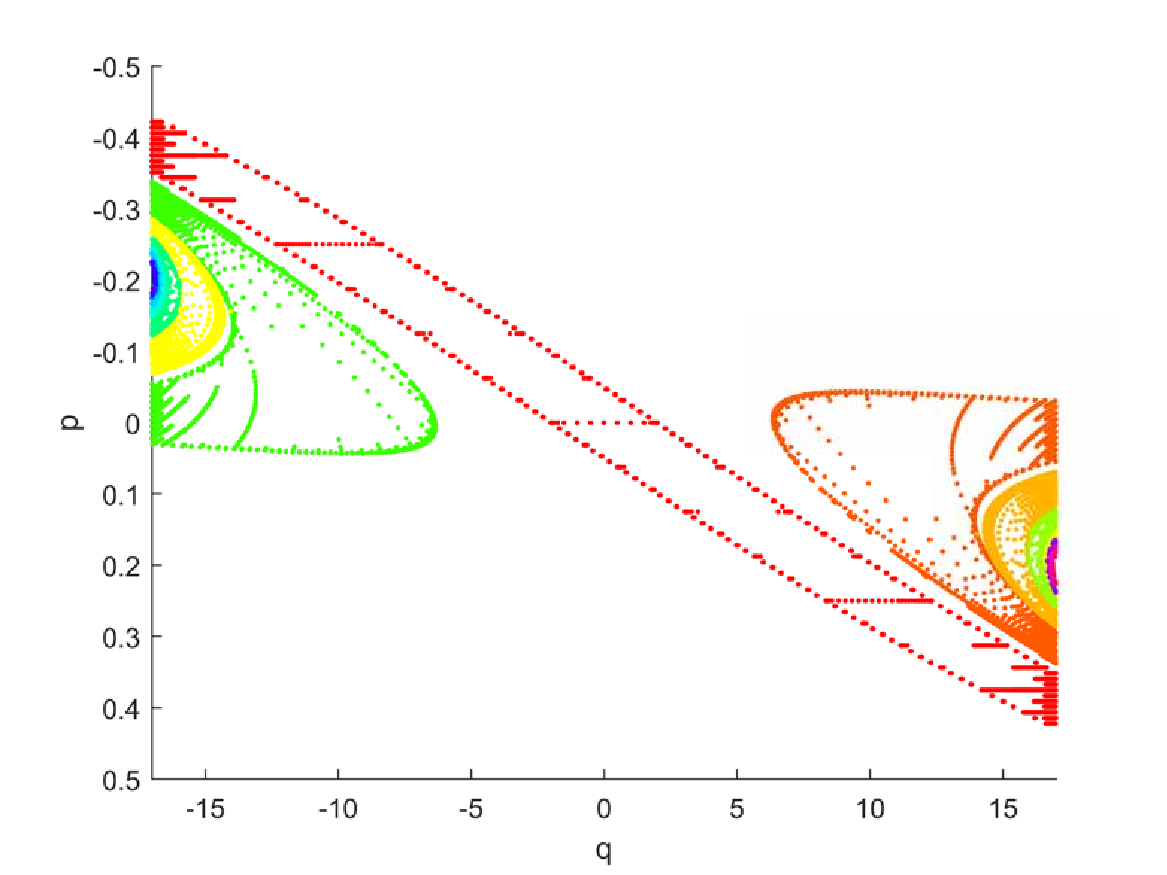
\includegraphics[width = \textwidth]{pr_target}
    \caption{Target PS \set{T}{}{} $= [-\variabile{b},\variabile{b}]\times[-1,1]$}
    \label{fig:target_triang_pr}
\end{subfigure}
\caption{\textbf{Rays distribution at \set{S}{}{} and \set{T}{}{} of the parabolic reflector.} Around $8300$ rays are traced using PS ray tracing with parameters $\varepsilon_{\variabile{q}_1}^{\textrm{min}} = 0.025, \; \varepsilon_{\variabile{q}_1}^{\textrm{max}} = 0.5, \; \varepsilon_{\variabile{p}_1}^{\textrm{max}} = \varepsilon_{\variabile{q}_1}^{\textrm{min}}/2, \mbox{ and }  \varepsilon_{\variabile{p}_1}^{\textrm{min}} = \varepsilon_{\variabile{q}_1}^{\textrm{max}}/2$ . $17$ different paths are found, each of them correspond to a certain number of reflections.}
 \label{fig:phase_space_pr}
\end{figure} The distribution of the rays in PS gives information about the paths they follow. We note that for the parabolic reflector many paths are found. Every path corresponds to a given number of reflections. Rays can have multiple reflections at lines $2$ and $3$ before arriving at the target. The parameters used in the triangulation refinement establish not only the number of rays traced but also the number of paths detected. For instance, for the values of the parameters defined above, the triangulation refinement is able to detect $17$ different paths. This means that up to $8$ multiple reflections occur between the rays and the two mirrors. Counting the number of rays that follow a given path $\Pi$, we can calculate the fraction of rays for every path. For example, tracing around $8300$ rays, the percentage of the rays that have $8$ multiple reflections along one of the two reflectors is around $0.13\%$. Rays that reflect many times before reaching the target do not give a significant contribution to the target intensity. Decreasing the value of the parameter $\varepsilon_{\variabile{q}_1}^{\textrm{min}}$, more paths can be found. The more reflections occur the smaller the correspond area in PS is. In order to find as many path as possible, also the parameter $\varepsilon_{\variabile{q}_1}^{\textrm{max}}$ needs to be decreased. Increasing the number of reflections considered, the corresponding regions in PS become smaller and smaller, see Figure \ref{fig:phase_space_pr}. \\ \indent Like for the optical systems considered in the previous sections, a stopping criterion of the triangulation refinement is determined for the parabolic reflector. Etendue conservation is used in order to find the values of the parameters that give a good approximation of the boundaries of the regions with positive luminance in PS. For the parabolic reflector in Figure \ref{fig:PR} all the rays that leave the source arrive at the target. Indeed, line $2$ and $3$ can only reflect rays (refraction law is not involved) and the target \'{e}tendue is equal to the source \'{e}tendue. From Equation (\ref{eq:etenduesource1}) we obtain:
\begin{equation}
U = U_1 = 4(\variabile{a}-\varepsilon)\approx 8.
\end{equation}
A range of values of $\varepsilon_{\variabile{q}_1}^{\textrm{min}}$ and $\varepsilon_{\variabile{q}_1}^{\textrm{max}}$ is considered (the triangulation parameters for the $\variabile{p}$-axis depend on the $\variabile{q}$-axis parameters according to Equation (\ref{eq:scaled_parameters})). For each couple of values, an approximation of the boundaries $\partial$\set{R}{}{}$(\Pi)$ is found for every path $\Pi$ as explained. $U_{\textrm{t}}$ is calculated for the approximated boundaries using Equation (\ref{eq:etenduetarg}). In Table \ref{tab:etendue_pr} we show how the number of rays traced, the paths found and the value for the target \'{e}tendue depend on the triangulation parameters.
We observe that, decreasing $\varepsilon_{\variabile{q}_1}^{\textrm{min}}$ and $\varepsilon_{\variabile{q}_1}^{\textrm{max}}$ the number of both the rays traced and the paths found increases. A maximum of $17$ different paths are detected. Furthermore, the value of $U_{\textrm{t}}$ gets closer and closer to the exact \'{e}tendue $U$.
\begin{table}[t] 
\centering
\caption{\bf Results of the triangulation refinement.}
\begin{tabular}{lllll}
 \hline   $\varepsilon_{\variabile{q}}^{\textrm{min}} $  & $\varepsilon_{\variabile{q}}^{\textrm{max}}$ & $\nrays$ & $\npath$ & Etendue \\
  \hline 
 $0.2$ & $1$   & $643$   &  $11$ & $5.71$\\
$0.1$ & $1$   & $1\,573$   &  $15$ & $7.23$\\
$0.025$  & $0.5$    & $8\,357$  & $17$ & $7.65$\\
 $0.025/2$  & $0.5/2$  & $18\,613$   & $17$ & $7.82$\\
$0.025/4$  & $0.5/4$  & $40\,465$   & $17$ & $7.82$\\
 $0.025/8$ & $0.5/8$  & $86\,529$    & $17$ & $7.96$\\
$0.025/16$ & $0.5/16$  & $185\,581$    & $17$ & $7.98$\\
 \hline
 \end{tabular}
 \label{tab:etendue_pr}
 \end{table}
\\ \indent Using the triangulation refinement that gives the best \'{e}tendue approximation, we calculate the target PS intensity $\hat{I}_{\textrm{PS}}$ from Equation (\ref{eq:PSintensity}).
The intensity profile is shown with the red line in Figure \ref{fig:intensity_pr}. The PS intensity is compared to a reference intensity $\hat{I}_{\textrm{ref}}$, computed using QMC ray tracing with $10^7$ rays. $\hat{I}_{\textrm{ref}}$ is depicted Figure \ref{fig:intensity_pr} with the dotted blue line. The graph shows that the two intensities coincide.
 \begin{figure}[t]
  \center
  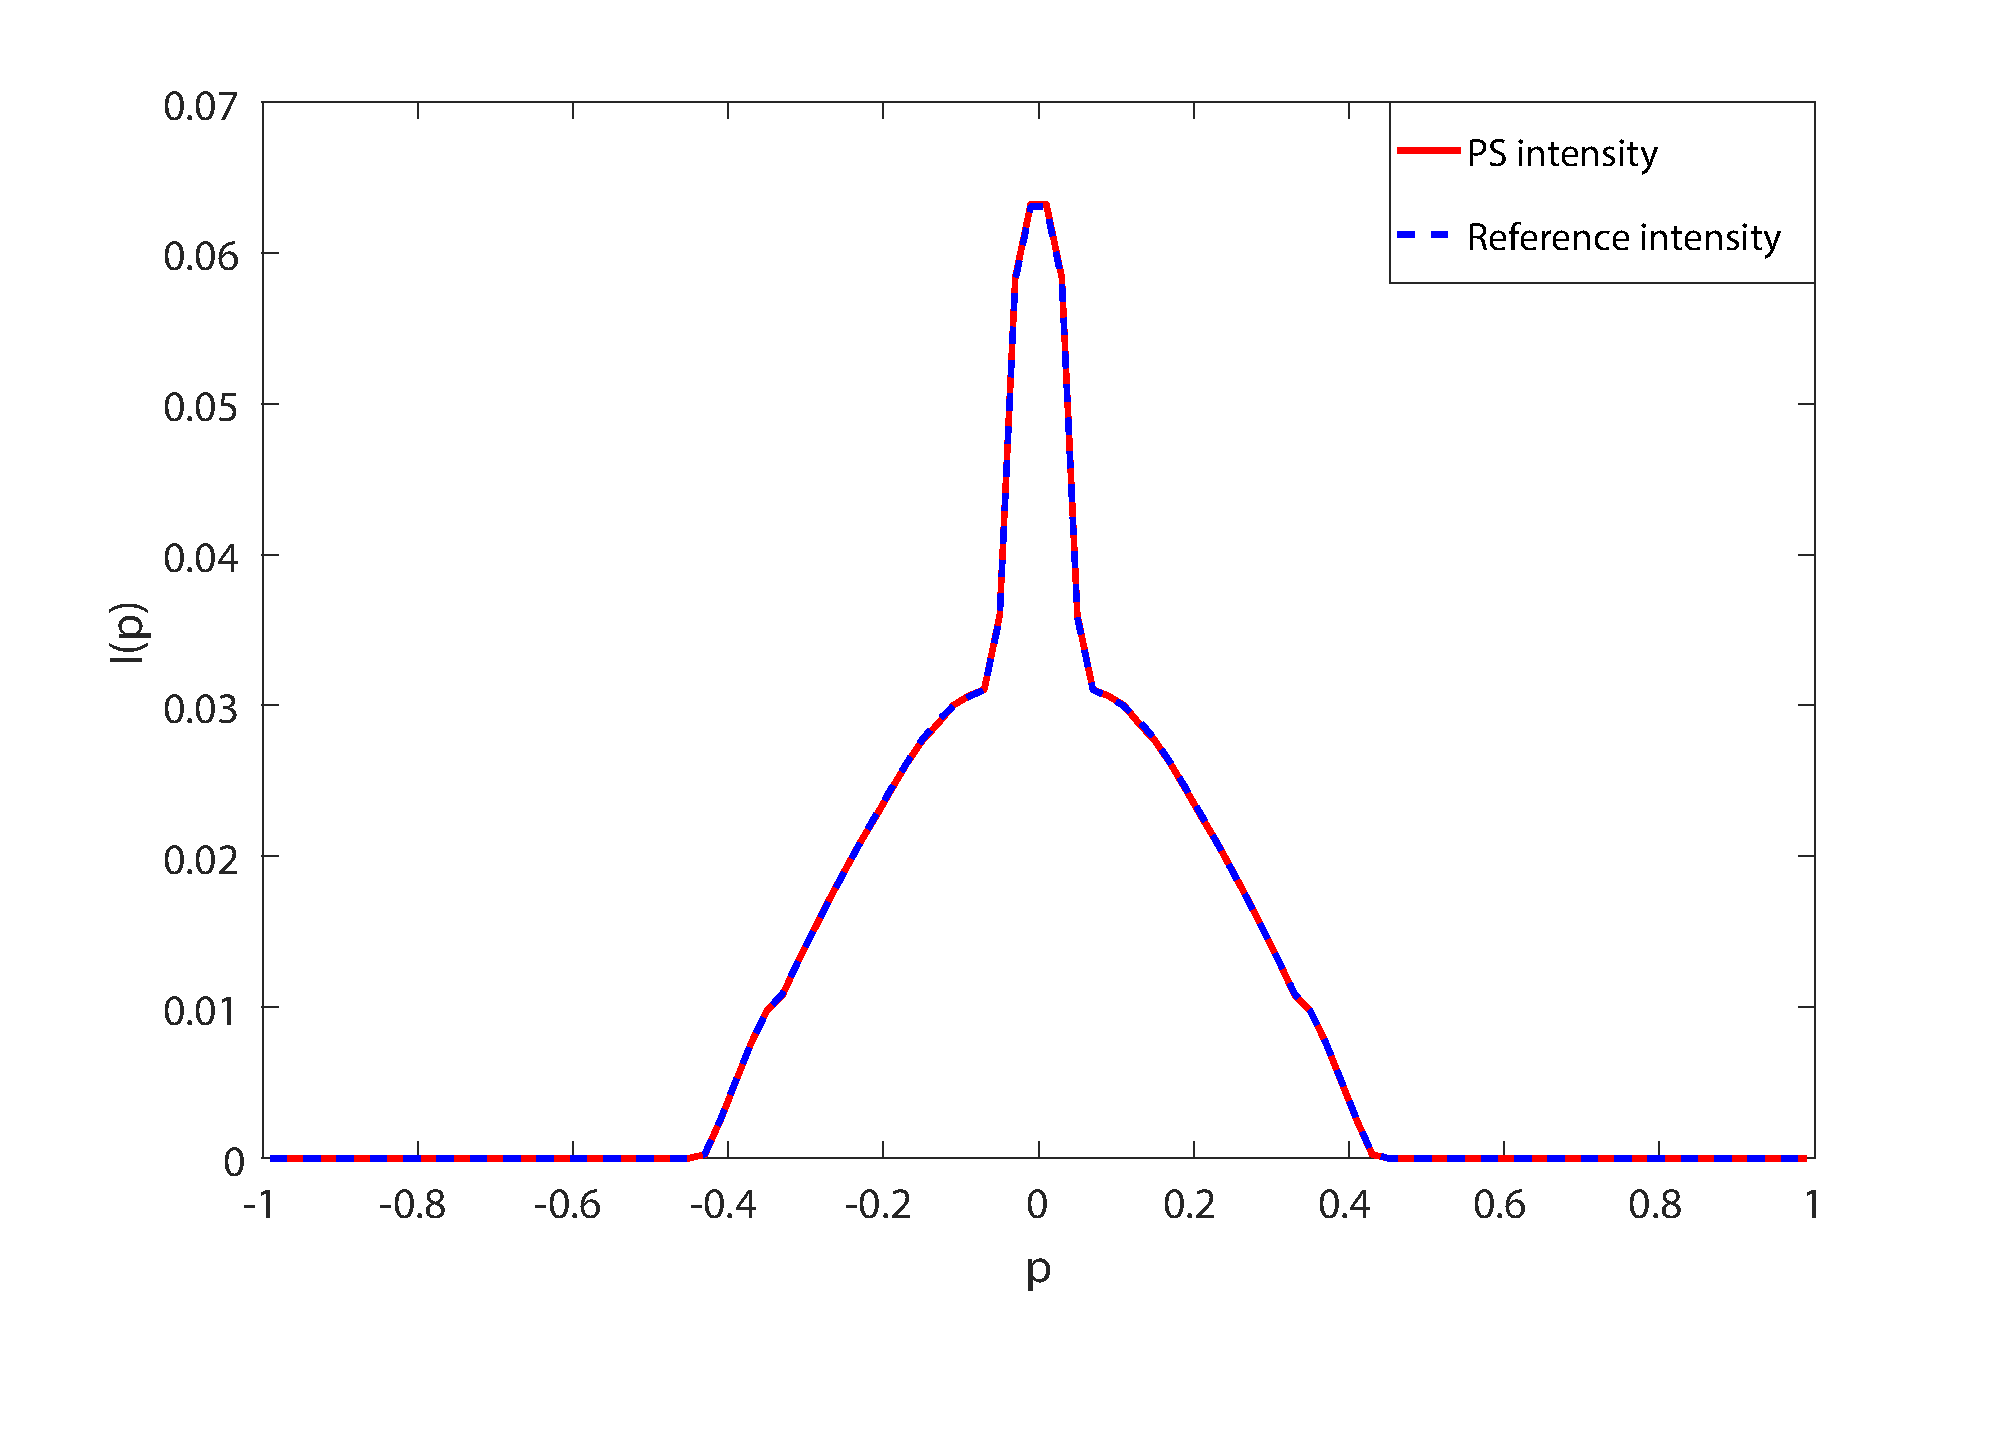
\includegraphics[width = \textwidth]{intensity_pr}
  \caption{\textbf{Target intensity of the parabolic reflector.} For the PS intensity the parameters $\varepsilon_{\variabile{q}_1}^{\textrm{min}}=1.56\cdot 10^{-3}$, $\varepsilon_{\variabile{q}_1}^{\textrm{max}}=3.13\cdot 10^{-2}$, $\varepsilon_{\variabile{p}_1}^{\textrm{min}}=\varepsilon_{\variabile{q}_1}^{\textrm{min}}/2$, and $\varepsilon_{\variabile{p}_1}^{\textrm{max}}=\varepsilon_{\variabile{q}_1}^{\textrm{max}}/2$ are used. Around $8.15 \cdot 10^{4}$ rays are traced in PS. For the reference intensity QMC ray tracing with $10^7$ rays is implemented.}
  \label{fig:intensity_pr}
\end{figure}
\begin{table}[t] \label{tab:table_pr_triangulation}
\centering
\caption{\bf Errors of the PS intensity for the parabolic reflector}
\begin{tabular}{lll}
 \hline   $\nrays$ & PS error & CPU-time (sec.) \\
  \hline 
 $643$        & $5.18\cdot10^{-4}$ & $0.24$\\
 $1\,573$       & $8.99\cdot 10^{-4}$ & $0.48$\\
 $8\,357$     & $2.87\cdot 10^{-4}$ & $2.40$ \\
 $18\,613$     & $1.38\cdot 10^{-4}$ & $5.48$\\
 $40\,465$   & $5.80\cdot 10^{-5}$ & $16.14$\\
 $86\,529$    & $2.90\cdot 10^{-5}$ & $55.04$\\
 $185\,581$   & $1.66\cdot 10^{-5}$ & $245.97$\\
 \hline
 \end{tabular}
\label{tab:table_pr_triangulation}
 \end{table}
\\ \indent 
Now, our method is compared to both MC and QMC ray tracing. 
The error between the approximate intensities $\hat{I}_{\textrm{A}}(\textrm{A}=\textrm{PS}, \textrm{MC}, \textrm{QMC})$ and the reference intensity is calculated. In Figure \ref{fig:error_rays_pr} the error as a function of the number of rays traced is shown for the three methods.
The green line represents the MC error, the blue line pictures the QMC error and the red line depicts the PS error. The errors are shown in a logarithmic scale, the dotted black line has slope $-1/2$, the dotted blue line has slope $-1$. Like for the other systems, MC ray tracing converges proportionally to $1/\sqrt{\nrays}$. QMC convergence is proportional to $1/\nrays$ for $\nrays \rightarrow \infty$. Less rays compared to MC ray tracing are needed in PS. In particular, to achieve an error of $10^{-4}$, around $10$ times less rays in PS are needed compared to MC and few rays less than QMC.
\begin{figure}[t]
  \center
  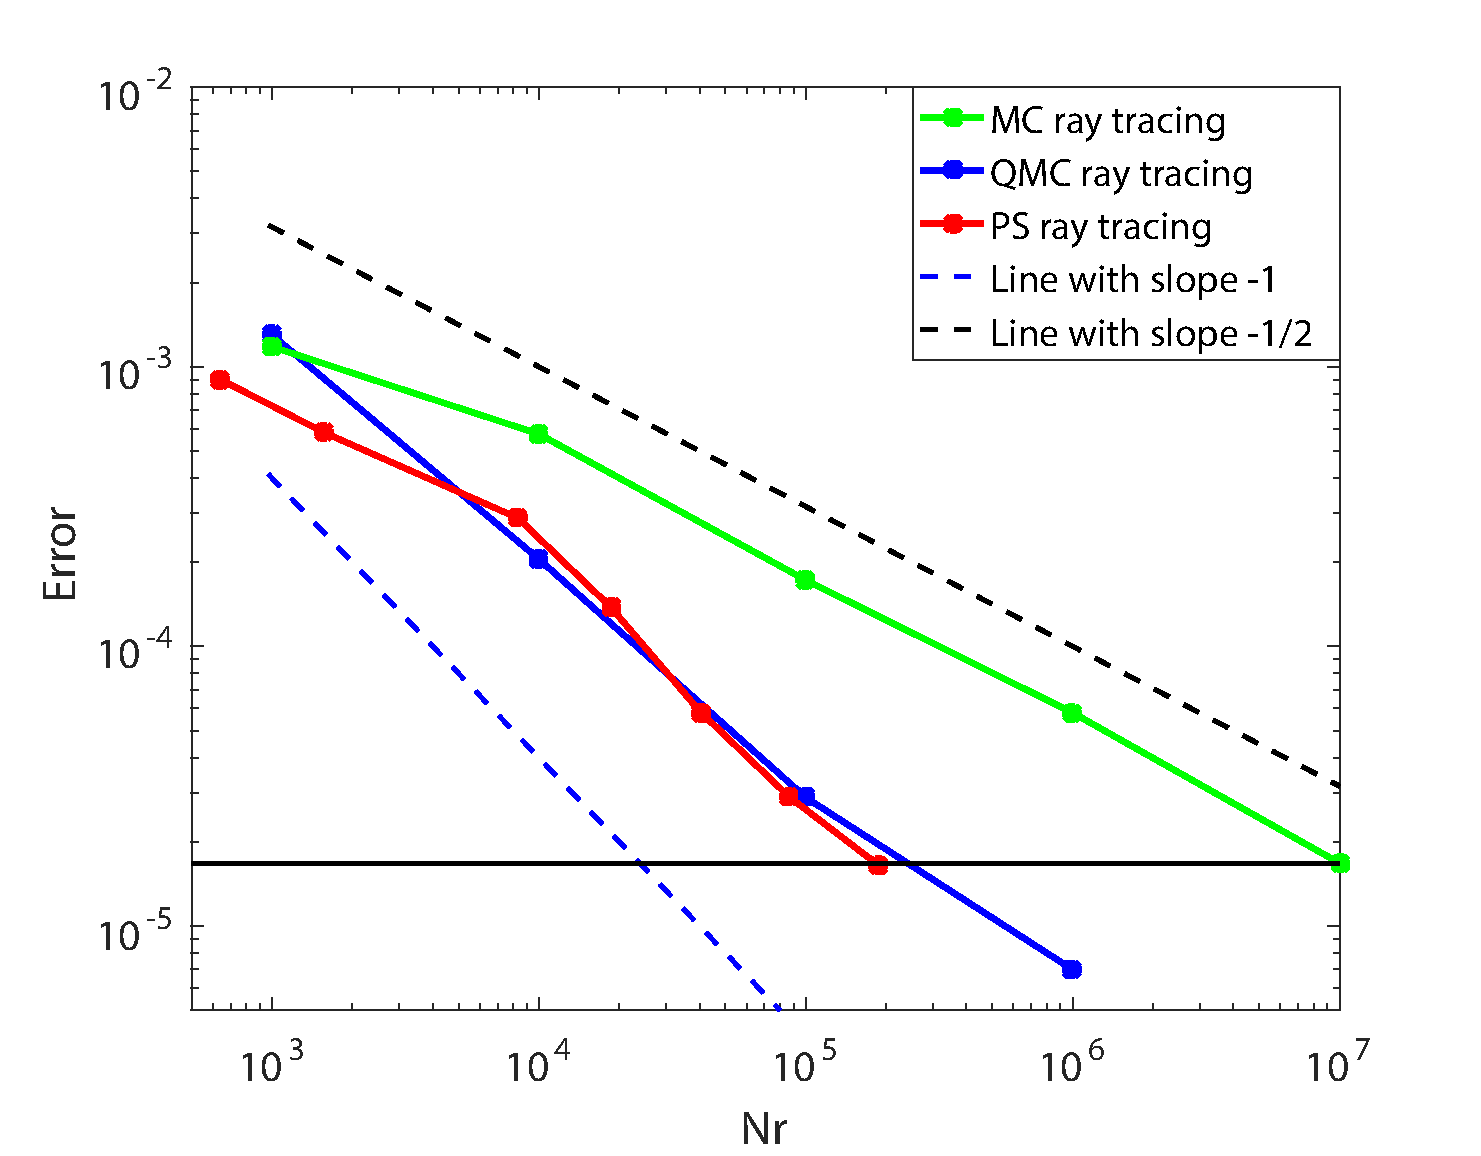
\includegraphics[width = \textwidth]{error_pr_100bin_rays}
  \caption{\textbf{Error as a function of the number of rays traced.} Less rays are needed using PS ray tracing compared to both MC and QMC ray tracing.}
  \label{fig:error_rays_pr}
\end{figure} 
\\ \indent
Finally, the error as a function of the CPU-time is shown in Figure \ref{fig:error_time_pr}. The MC, QMC and PS errors are depicted with the green, blue and red line, respectively. To obtain an error of the order of $10^{-5}$, PS ray tracing is $10$ times faster than MC ray tracing while becomes twice slower than QMC ray tracing. The detailed results of the numerical simulations are reported in Tables \ref{tab:mc_error_pr_triangulation} and \ref{tab:QMC_error_pr_triangulation}.
\begin{figure}[t]
  \center
  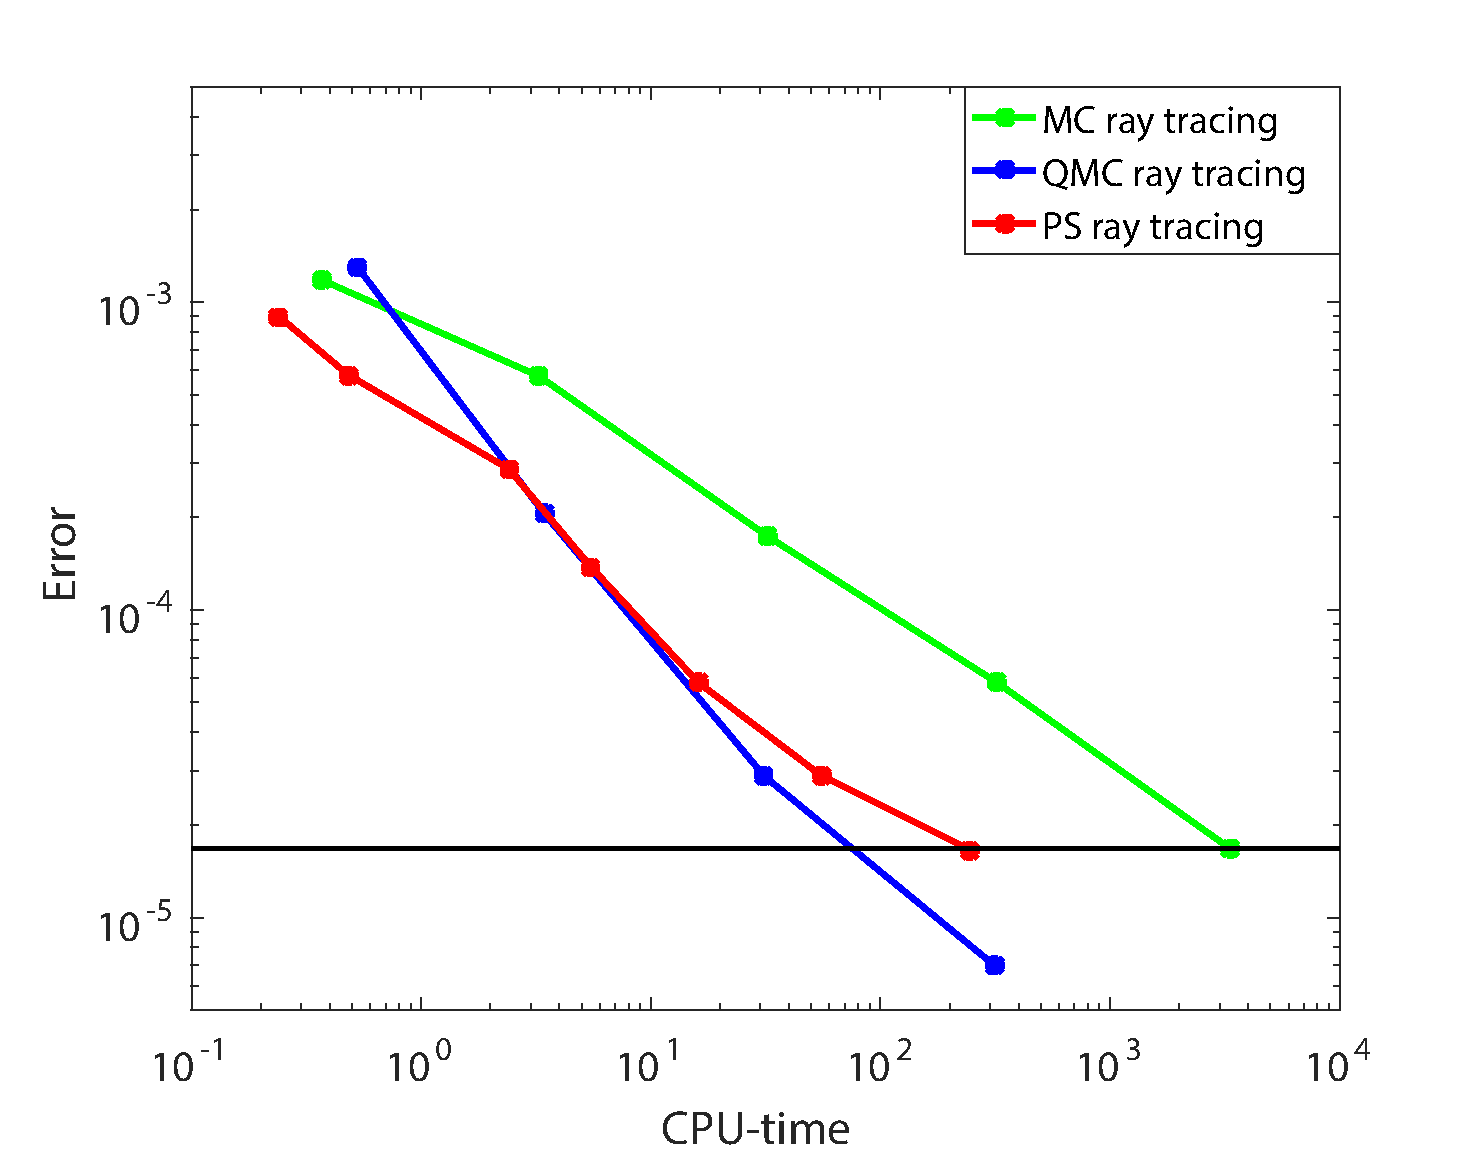
\includegraphics[width = \textwidth]{error_pr_100bin_time}
  \caption{\textbf{Error as a function of the CPU-time.} PS ray tracing has significant advantages in terms of the CPU-time compared to MC ray tracing. For the parabolic reflector the computational time is comparable with QMC ray tracing.}
  \label{fig:error_time_pr}
\end{figure} 
\begin{table}[t] 
\centering
\caption{\bf Errors of the MC intensity for the parabolic reflector}
\begin{tabular}{lll}
 \hline   $\nrays$ & MC error & CPU-time (sec.) \\
  \hline 
 $10^3$     & $1.18\cdot10^{-3}$ & $0.39$\\
 $10^4$     & $5.74\cdot 10^{-4}$ & $3.43$ \\
 $10^5$     & $1.73\cdot 10^{-4}$ & $33.13$\\
 $10^6$     & $5.79\cdot 10^{-5}$ & $328.96$\\
 $10^7$     & $1.68\cdot 10^{-5}$ & $3325.39$\\
 \hline
 \end{tabular}
 \label{tab:mc_error_pr_triangulation}
 \end{table}
\begin{table}[t] 
\centering
\caption{\bf Errors of the QMC intensity for the parabolic reflector}
\begin{tabular}{lll}
 \hline   $\nrays$ & QMC error & CPU-time (sec.) \\
  \hline 
 $10^3$     & $1.36\cdot10^{-3}$ & $0.53$\\
 $10^4$     & $2.05\cdot 10^{-4}$ & $3.44$ \\
 $10^5$     & $2.89\cdot 10^{-5}$ & $31.22$\\
 $10^6$     & $6.96\cdot 10^{-6}$ & $314.59$\\
 \hline
 \end{tabular}
 \label{tab:QMC_error_pr_triangulation}
 \end{table}
\\ \indent As explained above, MC and QMC errors also depend on the number of bins $\nbin$. In the simulations shown in this chapter we have always considered $\nbin = 100$. On the contrary, PS ray tracing calculates the intensity pointwise, nevertheless we considered $\nbin = 100$ bins at the target and we calculate the averaged normalized PS intensity over every bin in order to have a precise comparison with the binning procedures. Because of this, we expect that increasing the number of bins, the average PS intensity becomes more accurate. To verify this conjecture, we implemented MC, QMC and PS ray tracing considering a partitioning of the interval $[-1,1]$ into $\nbin = 150$ bins. The number of rays considered for the reference intensity have to be increased $(1.5)^5$ times. The averaged normalized intensities $\hat{I}_{\textrm{A}} (\textrm{A}=\textrm{MC}, \textrm{QMC}, \textrm{PS})$ found considering $\nbin=150$ bins are compared with the reference intensity $\hat{I}_{\textrm{ref}}$ (averaged and normalized) which is computed using QMC ray tracing with $7.6\cdot10^7$ rays. The error as a function of the number of rays is shown in Figure \ref{fig:error_pr_150_bin}. The results show that, using PS ray tracing an error of the order of $10^{-5}$ is obtained tracing around $10^2$ times less rays than MC ray tracing and twice less rays than QMC ray tracing. We conclude that, increasing the number of bins, PS error outperforms both MC and QMC ray tracing (see also Figure \ref{fig:error_rays_pr}).
\begin{figure}[h]
  \center
  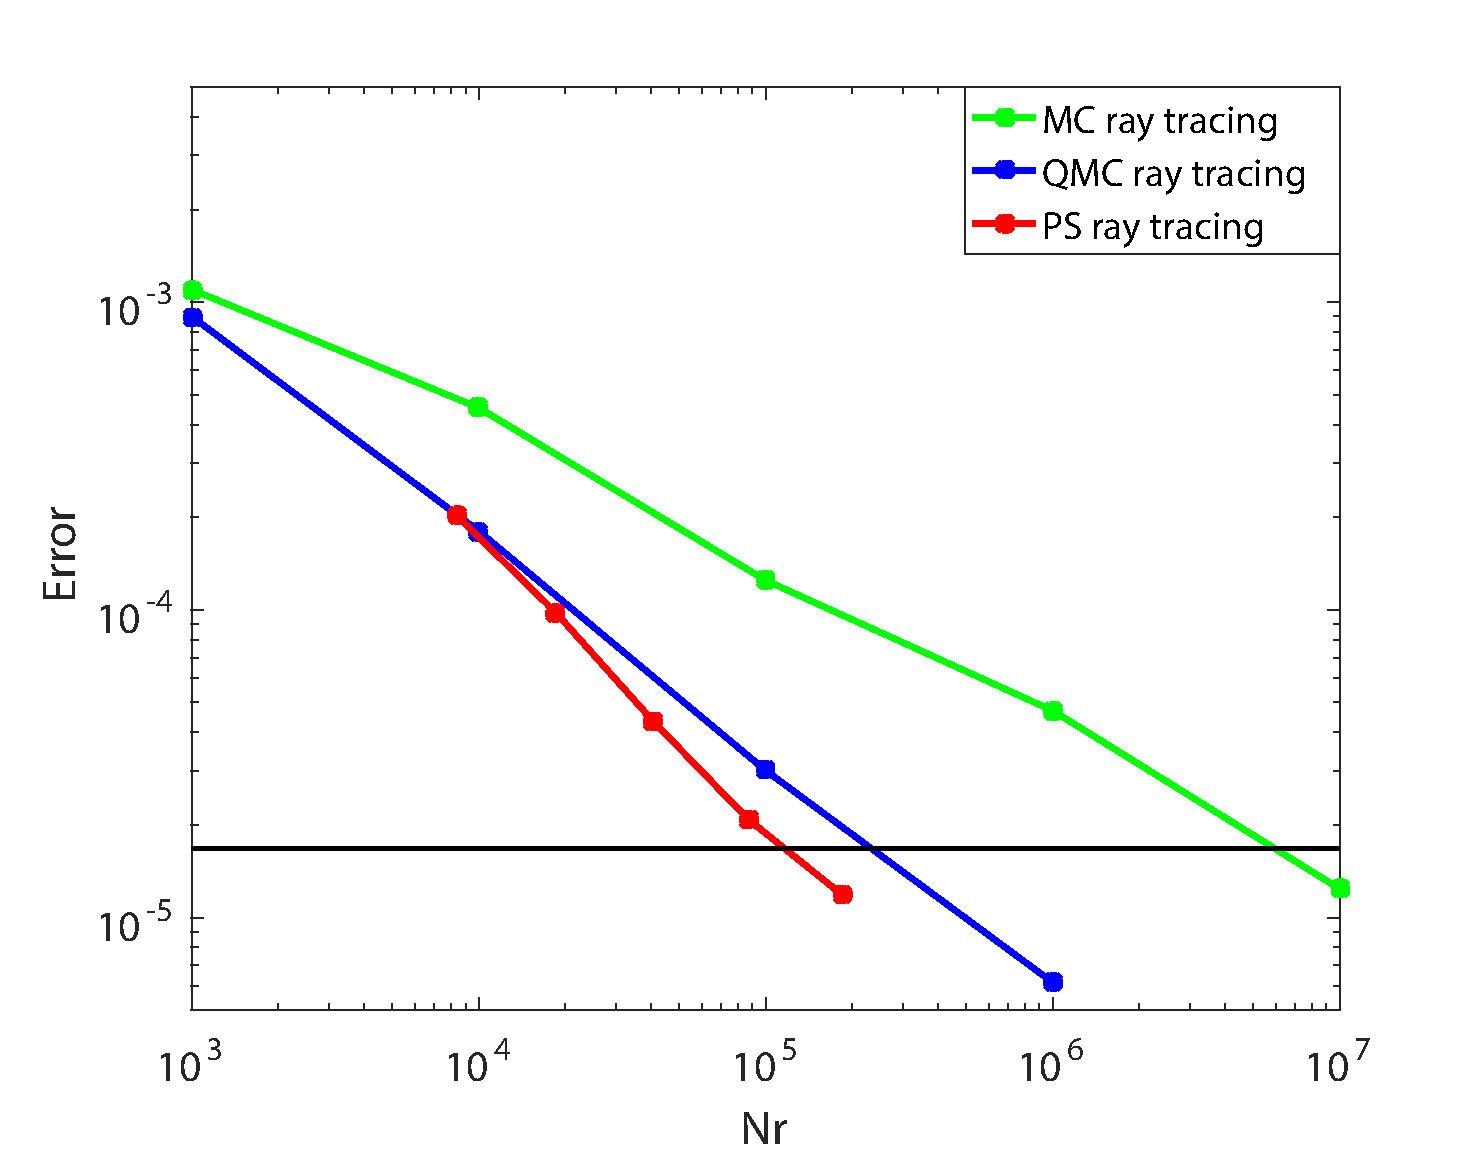
\includegraphics[width= \textwidth]{error_pr_150bins_ray}
  \caption{\textbf{Error plot for the parabolic reflector considering $\nbin=150$ bins.} Increasing the number of bins, the PS error decreases resulting in a better convergence compared to MC and QMC ray tracing.}
  \label{fig:error_pr_150_bin}
\end{figure}
\section{Discussion and conclusions}
In this chapter we presented a method to calculate the boundaries of the regions with positive luminance in PS. This method does not depend on the parameter $\alpha$ needed for the $\alpha$-shapes method presented in Chapter \ref{chap:boundaries_alpha}. Indeed, given a triangulation at the source PS, the boundaries are computed connecting the vertices of the boundary triangles, i.e., triangles crossed by a boundary, that follow the same path. Employing \'{e}tendue conservation, a stopping criterion for the triangulation refinement was developed. We applied the method to three different optical systems: the two-faceted cup, a TIR-collimator, and a parabolic reflector. Numerical results show that PS ray tracing is faster and more accurate than MC ray tracing. Compared to QMC ray tracing we observed accuracy and speed advantages of an order of magnitude with our method for the TIR-collimator. 
For the two-faceted cup, PS ray tracing has a slower convergence compared to QMC ray tracing. For the parabolic reflector PS and QMC ray tracing display similar convergence. As an example, for this system we showed that increasing the number of bins the errors decrease. 
To conclude we state that QMC ray tracing performs better than PS ray tracing for very simple optical systems, but the PS approach is more suitable for complicated optical systems.
\\ \indent In order to further improve PS ray tracing we develop a new method which employs the PS of \textit{all} the optical lines. This method is explained in the next chapter.
%We claim that PS ray tracing is also more accurate than the ray tracing procedure proposed by Moore (2013), \cite{moore2013methods}.
%The novelty of our approach compared to the method used by Moore, is briefly explained below. First, to compute the output intensity, we employ the phase space of the target. This avoids the use of any interpolation to compute the photometric variables and therefore, more accurate results are obtained.
%Second, in  all rays that leave the source start at the same position and only a sampling angular range is given. In our approach a rectangular source is considered thus, both the angular and spatial coordinates of each ray change. This extra variable can produce very irregular shapes of the regions at target phase space. To overcome this issue, we employ the edge-ray principle and we consider the regions at source phase space where the distribution of the rays is much more regular and the corresponding boundaries are easily computed.
%As a consequence, our procedure is suitable to compute the output intensity as function of both the angular or the spatial coordinates.
%Third, using the conservation of \'{e}tendue, we provided a criterion to stop the triangulation refinement. In this way we can estimate the number of rays required to obtain the desired accuracy and thus, we avoid tracing more rays than necessary.









 

%\section{The Compound Parabolic Concentrator (CPC)}